\documentclass[openany]{book}
\usepackage{lmodern}
\usepackage{amssymb,amsmath}
\usepackage{ifxetex,ifluatex}
\usepackage{fixltx2e} % provides \textsubscript
\ifnum 0\ifxetex 1\fi\ifluatex 1\fi=0 % if pdftex
  \usepackage[T1]{fontenc}
  \usepackage[utf8]{inputenc}
\else % if luatex or xelatex
  \ifxetex
    \usepackage{mathspec}
  \else
    \usepackage{fontspec}
  \fi
  \defaultfontfeatures{Ligatures=TeX,Scale=MatchLowercase}
\fi
% use upquote if available, for straight quotes in verbatim environments
\IfFileExists{upquote.sty}{\usepackage{upquote}}{}
% use microtype if available
\IfFileExists{microtype.sty}{%
\usepackage{microtype}
\UseMicrotypeSet[protrusion]{basicmath} % disable protrusion for tt fonts
}{}
\usepackage{hyperref}
\hypersetup{unicode=true,
            pdftitle={DATA 624: Project 1},
            pdfauthor={Vinicio Haro; Sang Yoon (Andy) Hwang; Julian McEachern; Jeremy O'Brien; Bethany Poulin},
            pdfborder={0 0 0},
            breaklinks=true}
\urlstyle{same}  % don't use monospace font for urls
\usepackage{natbib}
\bibliographystyle{plainnat}
\usepackage{color}
\usepackage{fancyvrb}
\newcommand{\VerbBar}{|}
\newcommand{\VERB}{\Verb[commandchars=\\\{\}]}
\DefineVerbatimEnvironment{Highlighting}{Verbatim}{commandchars=\\\{\}}
% Add ',fontsize=\small' for more characters per line
\usepackage{framed}
\definecolor{shadecolor}{RGB}{248,248,248}
\newenvironment{Shaded}{\begin{snugshade}}{\end{snugshade}}
\newcommand{\AlertTok}[1]{\textcolor[rgb]{0.94,0.16,0.16}{#1}}
\newcommand{\AnnotationTok}[1]{\textcolor[rgb]{0.56,0.35,0.01}{\textbf{\textit{#1}}}}
\newcommand{\AttributeTok}[1]{\textcolor[rgb]{0.77,0.63,0.00}{#1}}
\newcommand{\BaseNTok}[1]{\textcolor[rgb]{0.00,0.00,0.81}{#1}}
\newcommand{\BuiltInTok}[1]{#1}
\newcommand{\CharTok}[1]{\textcolor[rgb]{0.31,0.60,0.02}{#1}}
\newcommand{\CommentTok}[1]{\textcolor[rgb]{0.56,0.35,0.01}{\textit{#1}}}
\newcommand{\CommentVarTok}[1]{\textcolor[rgb]{0.56,0.35,0.01}{\textbf{\textit{#1}}}}
\newcommand{\ConstantTok}[1]{\textcolor[rgb]{0.00,0.00,0.00}{#1}}
\newcommand{\ControlFlowTok}[1]{\textcolor[rgb]{0.13,0.29,0.53}{\textbf{#1}}}
\newcommand{\DataTypeTok}[1]{\textcolor[rgb]{0.13,0.29,0.53}{#1}}
\newcommand{\DecValTok}[1]{\textcolor[rgb]{0.00,0.00,0.81}{#1}}
\newcommand{\DocumentationTok}[1]{\textcolor[rgb]{0.56,0.35,0.01}{\textbf{\textit{#1}}}}
\newcommand{\ErrorTok}[1]{\textcolor[rgb]{0.64,0.00,0.00}{\textbf{#1}}}
\newcommand{\ExtensionTok}[1]{#1}
\newcommand{\FloatTok}[1]{\textcolor[rgb]{0.00,0.00,0.81}{#1}}
\newcommand{\FunctionTok}[1]{\textcolor[rgb]{0.00,0.00,0.00}{#1}}
\newcommand{\ImportTok}[1]{#1}
\newcommand{\InformationTok}[1]{\textcolor[rgb]{0.56,0.35,0.01}{\textbf{\textit{#1}}}}
\newcommand{\KeywordTok}[1]{\textcolor[rgb]{0.13,0.29,0.53}{\textbf{#1}}}
\newcommand{\NormalTok}[1]{#1}
\newcommand{\OperatorTok}[1]{\textcolor[rgb]{0.81,0.36,0.00}{\textbf{#1}}}
\newcommand{\OtherTok}[1]{\textcolor[rgb]{0.56,0.35,0.01}{#1}}
\newcommand{\PreprocessorTok}[1]{\textcolor[rgb]{0.56,0.35,0.01}{\textit{#1}}}
\newcommand{\RegionMarkerTok}[1]{#1}
\newcommand{\SpecialCharTok}[1]{\textcolor[rgb]{0.00,0.00,0.00}{#1}}
\newcommand{\SpecialStringTok}[1]{\textcolor[rgb]{0.31,0.60,0.02}{#1}}
\newcommand{\StringTok}[1]{\textcolor[rgb]{0.31,0.60,0.02}{#1}}
\newcommand{\VariableTok}[1]{\textcolor[rgb]{0.00,0.00,0.00}{#1}}
\newcommand{\VerbatimStringTok}[1]{\textcolor[rgb]{0.31,0.60,0.02}{#1}}
\newcommand{\WarningTok}[1]{\textcolor[rgb]{0.56,0.35,0.01}{\textbf{\textit{#1}}}}
\usepackage{longtable,booktabs}
\usepackage{graphicx,grffile}
\makeatletter
\def\maxwidth{\ifdim\Gin@nat@width>\linewidth\linewidth\else\Gin@nat@width\fi}
\def\maxheight{\ifdim\Gin@nat@height>\textheight\textheight\else\Gin@nat@height\fi}
\makeatother
% Scale images if necessary, so that they will not overflow the page
% margins by default, and it is still possible to overwrite the defaults
% using explicit options in \includegraphics[width, height, ...]{}
\setkeys{Gin}{width=\maxwidth,height=\maxheight,keepaspectratio}
\IfFileExists{parskip.sty}{%
\usepackage{parskip}
}{% else
\setlength{\parindent}{0pt}
\setlength{\parskip}{6pt plus 2pt minus 1pt}
}
\setlength{\emergencystretch}{3em}  % prevent overfull lines
\providecommand{\tightlist}{%
  \setlength{\itemsep}{0pt}\setlength{\parskip}{0pt}}
\setcounter{secnumdepth}{5}

%%% Use protect on footnotes to avoid problems with footnotes in titles
\let\rmarkdownfootnote\footnote%
\def\footnote{\protect\rmarkdownfootnote}

%%% Change title format to be more compact
\usepackage{titling}

% Create subtitle command for use in maketitle
\providecommand{\subtitle}[1]{
  \posttitle{
    \begin{center}\large#1\end{center}
    }
}

\setlength{\droptitle}{-2em}

  \title{DATA 624: Project 1}
    \pretitle{\vspace{\droptitle}\centering\huge}
  \posttitle{\par}
    \author{Vinicio Haro \\ Sang Yoon (Andy) Hwang \\ Julian McEachern \\ Jeremy O'Brien \\ Bethany Poulin}
    \preauthor{\centering\large\emph}
  \postauthor{\par}
      \predate{\centering\large\emph}
  \postdate{\par}
    \date{October 22, 2019}

\usepackage{booktabs}
\usepackage[table]{xcolor}

% set plain style for page numbers
\pagestyle{plain}
\raggedbottom

% change font
\usepackage{fontspec}
\setmainfont{Arial}

% remove "chapter" from chapter title
\usepackage{titlesec}
\titleformat{\chapter}
  {\normalfont\LARGE\bfseries}{\thechapter}{1em}{}
\titlespacing*{\chapter}{0pt}{3.5ex plus 1ex minus .2ex}{2.3ex plus .2ex}

% create color block quotes
\usepackage{tcolorbox}
\newtcolorbox{myquote}{colback=orange!05!white, colframe=black!75!black}
\renewenvironment{quote}{\begin{myquote}}{\end{myquote}}

% wrap text
\usepackage{geometry}[textwidth=6in]

% kable 
\usepackage{tabu}
\usepackage{float}
\usepackage{booktabs}
\usepackage{longtable}
\usepackage{array}
\usepackage{multirow}
\usepackage{wrapfig}
\usepackage{float}
\usepackage{colortbl}
\usepackage{pdflscape}
\usepackage{tabu}
\usepackage{threeparttable}
\usepackage{threeparttablex}
\usepackage[normalem]{ulem}
\usepackage{makecell}
\usepackage{xcolor}

\begin{document}
\maketitle

{
\setcounter{tocdepth}{1}
\tableofcontents
}
\hypertarget{overview}{%
\chapter*{Overview}\label{overview}}
\addcontentsline{toc}{chapter}{Overview}

We split the work into three sections for Project 1. Individual team
members each took lead on individual problem. Jeremey and Julian focused
on Part A, Sang Yoon (Andy) and Vinicio worked on Part B, and Bethany
took lead on Part C. Juliann created an overall format for the
assignment to be used and all team members collectively worked together
on reviewing and merging our finished product.

\hypertarget{dependencies}{%
\section*{Dependencies}\label{dependencies}}
\addcontentsline{toc}{section}{Dependencies}

The following R libraries were used to complete this assignment:

\begin{Shaded}
\begin{Highlighting}[]
\KeywordTok{library}\NormalTok{(easypackages)}

\KeywordTok{libraries}\NormalTok{(}\StringTok{'knitr'}\NormalTok{, }\StringTok{'kableExtra'}\NormalTok{, }\StringTok{'default'}\NormalTok{)}

\CommentTok{# Processing}
\KeywordTok{libraries}\NormalTok{(}\StringTok{'readxl'}\NormalTok{, }\StringTok{'tidyverse'}\NormalTok{, }\StringTok{'janitor'}\NormalTok{, }\StringTok{'imputeTS'}\NormalTok{, }\StringTok{'tsoutliers'}\NormalTok{, }\StringTok{'lubridate'}\NormalTok{, }\StringTok{'xlsx'}\NormalTok{)}

\CommentTok{# Timeseries }
\KeywordTok{libraries}\NormalTok{(}\StringTok{'psych'}\NormalTok{, }\StringTok{'urca'}\NormalTok{, }\StringTok{'forecast'}\NormalTok{, }\StringTok{'timetk'}\NormalTok{, }\StringTok{'fpp2'}\NormalTok{)}

\CommentTok{# Graphing}
\KeywordTok{libraries}\NormalTok{(}\StringTok{'ggplot2'}\NormalTok{, }\StringTok{'grid'}\NormalTok{, }\StringTok{'gridExtra'}\NormalTok{, }\StringTok{'ggfortify'}\NormalTok{,}\StringTok{'ggpubr'}\NormalTok{, }\StringTok{'scales'}\NormalTok{)}
\end{Highlighting}
\end{Shaded}

\hypertarget{data}{%
\section*{Data}\label{data}}
\addcontentsline{toc}{section}{Data}

Data was stored within our group repository and imported below using the
\texttt{readxl} package. Each individual question was solved within an R
script and the data was sourced into our main report. For replication
purposes, we also made our R scripts available within our appendix. All
forecasts have been exported and saved to a single \texttt{.xlsx} file
in our
\href{https://github.com/JeremyOBrien16/CUNY_DATA_624/tree/master/Project\%20One/}{github
repository} folder named forecasts.

\begin{Shaded}
\begin{Highlighting}[]
\CommentTok{# Data Aquisition}
\NormalTok{atm_data <-}\StringTok{ }\KeywordTok{read_excel}\NormalTok{(}\StringTok{"data/ATM624Data.xlsx"}\NormalTok{) }
\NormalTok{power_data <-}\StringTok{ }\KeywordTok{read_excel}\NormalTok{(}\StringTok{"data/ResidentialCustomerForecastLoad-624.xlsx"}\NormalTok{) }
\NormalTok{pipe1_data <-}\StringTok{ }\KeywordTok{read_excel}\NormalTok{(}\StringTok{"data/Waterflow_Pipe1.xlsx"}\NormalTok{)}
\NormalTok{pipe2_data <-}\StringTok{ }\KeywordTok{read_excel}\NormalTok{(}\StringTok{"data/Waterflow_Pipe2.xlsx"}\NormalTok{)}

\CommentTok{# Source Code}
\KeywordTok{source}\NormalTok{(}\StringTok{'~/GitHub/CUNY_DATA_624/Project One/scripts/Part-A.R'}\NormalTok{)}
\KeywordTok{source}\NormalTok{(}\StringTok{'~/GitHub/CUNY_DATA_624/Project One/scripts/Part-B.R'}\NormalTok{)}
\KeywordTok{source}\NormalTok{(}\StringTok{'~/GitHub/CUNY_DATA_624/Project One/scripts/Part-C.R'}\NormalTok{)}
\end{Highlighting}
\end{Shaded}

\hypertarget{part-a-atms}{%
\chapter{Part A: ATMs}\label{part-a-atms}}

\begin{quote}
\textbf{Instructions:} In part A, I want you to forecast how much cash
is taken out of 4 different ATM machines for May 2010. The data is given
in a single file. The variable \texttt{Cash} is provided in hundreds of
dollars, other than that, it is straight forward. I am being somewhat
ambiguous on purpose. I am giving you data, please provide your written
report on your findings, visuals, discussion and your R code all within
a Word readable document, except the forecast which you will put in an
Excel readable file. I must be able to cut and paste your R code and run
it in R studio. Your report must be professional - most of all -
readable, EASY to follow. Let me know what you are thinking, assumptions
you are making! Your forecast is a simple CSV or Excel file that MATCHES
the format of the data I provide.
\end{quote}

\hypertarget{exploration}{%
\section{Exploration}\label{exploration}}

The data covers a period of Friday May 1, 2010 through Saturday April
30, 2010. While reviewing the data, we identified that the original data
file contained \texttt{NA} values in our \texttt{ATM} and \texttt{Cash}
columns for 14 observations between May 1 and 14, 2010. As these contain
no information, we removed these missing values and transformed the
dataset into a wide format.

Our initial review also revealed that ATM2 contained one missing value
on 2009-10-25 and that ATM4 contained a potential outlier of \$1,123 on
2010-02-09. We replaced both values with the corresponding mean value of
each machine.

We examined summary statistics for each ATM time series (a table can be
found in the appendix).

\begin{itemize}
\tightlist
\item
  ATM1 and ATM2 have pretty normal distributions; ATM1's daily mean cash
  dispensed is \$84, and ATM2's is \$62.
\item
  ATM3 only dispensed cash on the last three days of the time series -
  as this provides few data points on which to forecast, we'll need to
  treat it specially.
\item
  ATM4 has a similar mean to ATM1, but skew and kurtosis suggest the
  impact of an outlier Wednesday, February 10, 2010. If this ATM is
  located in the Northeastern United States, this may have a
  relationship to a blizzard which struck on that day.
\end{itemize}

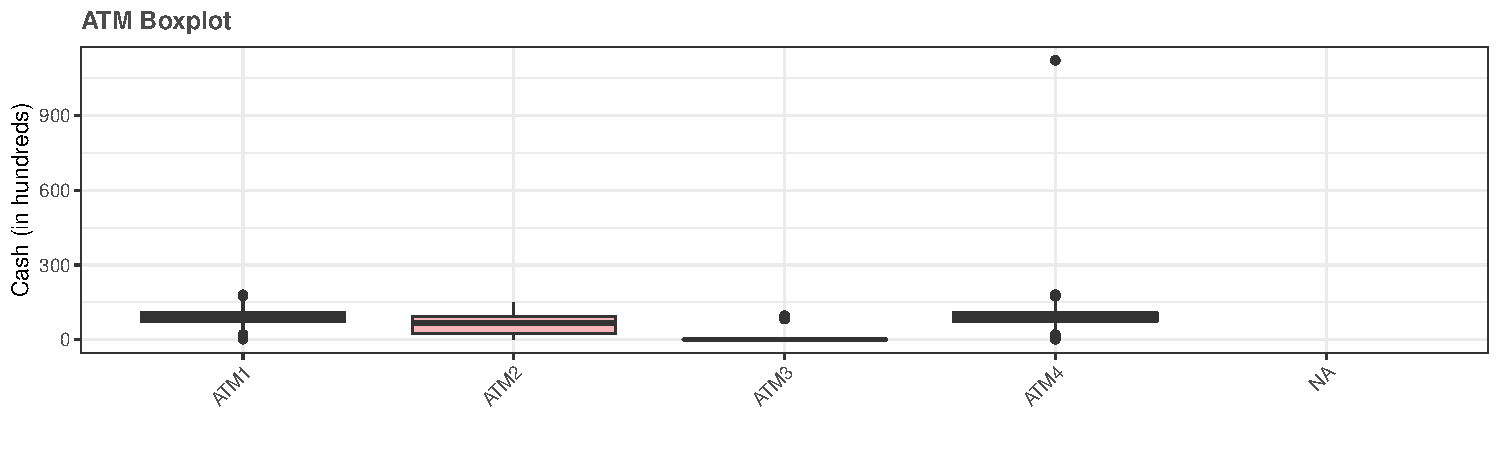
\includegraphics{Group2_Project1_Fall2019_files/figure-latex/unnamed-chunk-2-1.pdf}

Last, we used a scatterplot to examine the correlation between cash
withdrawals and dates for each machine. We identified similiar patterns
between ATM1 and ATM4, which show non-linear fluctuations that suggest a
potential trend component in these timeseries. ATM2 follows a relatively
linear path and decreases overtime. This changes in the last few
observations, where withdrawals begin to increase. As mentioned, there
are only 3 observed transactions for ATM3 that appear at the end of the
captured time period.

Our cleaned dataframe was then converted into a timeseries format. The
time series plots show high weekly variance, for ATM1, ATM2, and ATM4 -
consistent with our takeaway from the scatterplots.

These plots also remind us that ATM3 only dispensed cash on 3 days at
the end of the timespan, with a daily range between \$82 and \$96. Given
the paucity of observations in the training data, the simplest possible
approach to forecasting ATM3, averaging, is likely best. Given that ATM3
distributed no cash until April 28, 2010, we'll assume that it was not
operating until then and only include the three day window of non-zero
observations in the forecast.

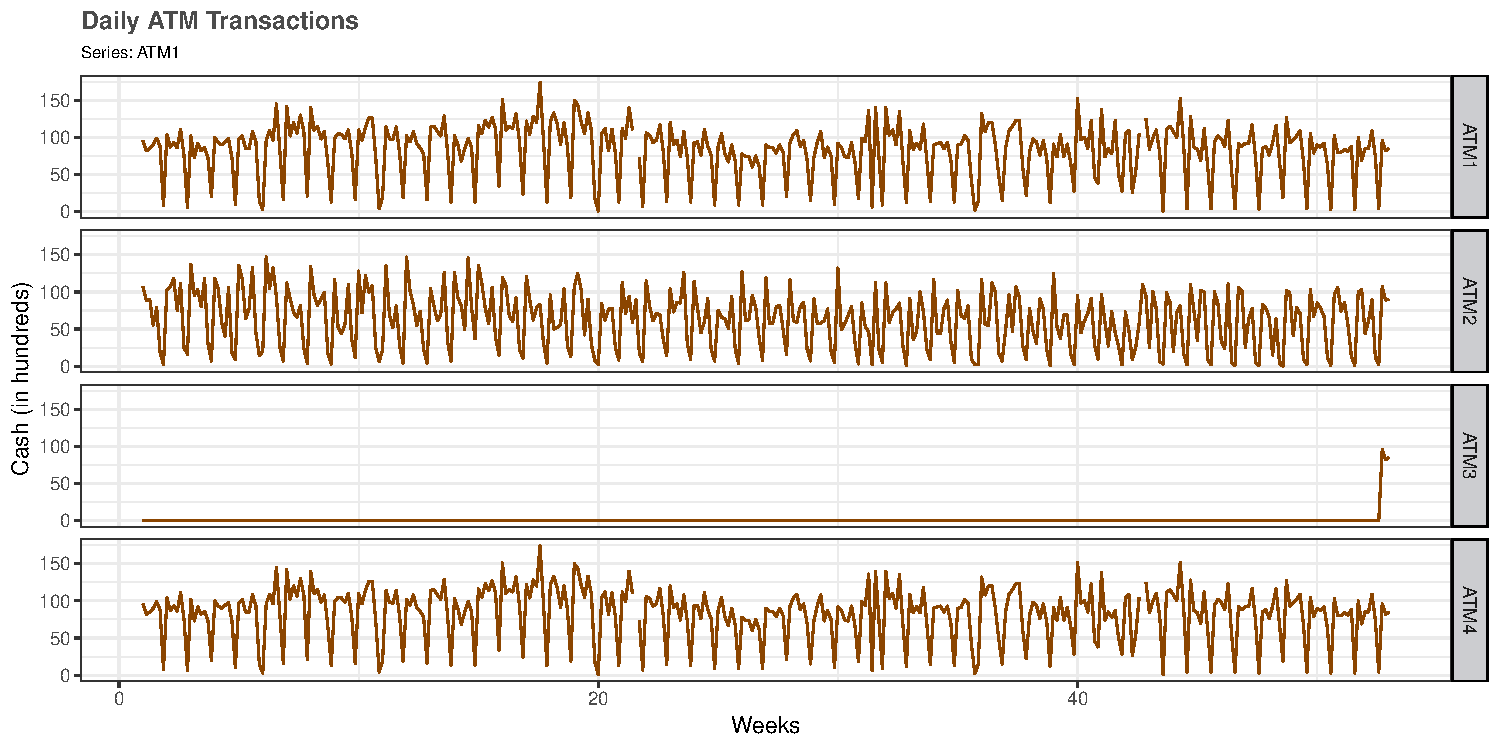
\includegraphics{Group2_Project1_Fall2019_files/figure-latex/unnamed-chunk-3-1.pdf}

\hypertarget{evaluation}{%
\section{Evaluation}\label{evaluation}}

We constructed our initial timeseries for ATM1, ATM2, and ATM4 using a
weekly frequency. Our ACF plots for each ATM showcases large, decreasing
lags starting at 7. This pattern continues in a multiple of seven, which
confirms our assumption about seasonality within the observed data.
These lags are indicative of a weekly pattern. \newline

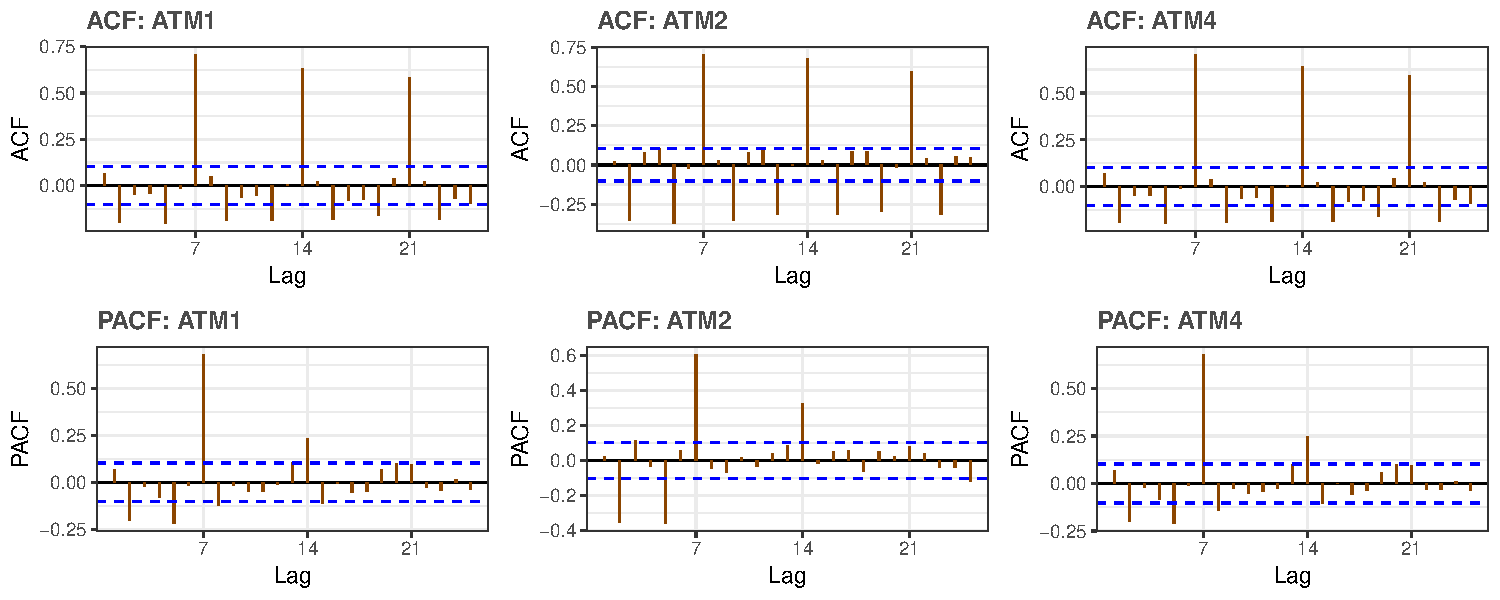
\includegraphics{Group2_Project1_Fall2019_files/figure-latex/unnamed-chunk-4-1.pdf}

Our plots further suggest that the ATM data is non-stationary. We
performed a unit root test using the \texttt{ur.kpss()} function to
confirm this observation. The test results below show that differencing
is required on all ATM2 and ATM4 series. ATM1 falls just below the
cut-off critical value, but could still benefit from differencing due to
the observed seasonal pattern.

\begin{table}[H]

\caption{\label{tab:unnamed-chunk-5}KPSS unit root test}
\centering
\begin{tabular}{l|l|l}
\hline
\textbf{ATM} & \textbf{No-Diff} & \textbf{Diff-1}\\
\hline
\rowcolor{gray!6}  ATM1 & 0.4967 & 0.0219\\
\hline
ATM2 & 2.0006 & 0.016\\
\hline
\rowcolor{gray!6}  ATM4 & 0.5182 & 0.0211\\
\hline
\end{tabular}
\end{table}

\hypertarget{modeling}{%
\section{Modeling}\label{modeling}}

We used \texttt{auto.arima()} and set \texttt{D=1} to account for
seasonal differencing of our data to select the best ARIMA models for
ATM1, ATM2, and ATM4. The full models and accuracy statistics for each
series can be viewed in the appendix.

\begin{itemize}
\tightlist
\item
  \textbf{ATM1}: ARIMA\((0,0,2)(0,1,1)_7\)
\item
  \textbf{ATM2}: ARIMA\((2,0,2)(0,1,1)_7\)
\item
  \textbf{ATM3}: MEAN
\item
  \textbf{ATM4}: ARIMA\((0,0,2)(0,1,1)_7\)
\end{itemize}

The residual ACF plots contain no pattern and the lags fall within the
critical value, which suggest they are white noise and not
autocorrelated. The residual histograms follow a relatively normal
distribution that is centered around zero. The p-value from the
Ljung-Box test for ATM1, ATM2, and ATM4 all exceeds 0.05, which futher
supports that residuals happen by chance and the models adequately fit
the observed data.

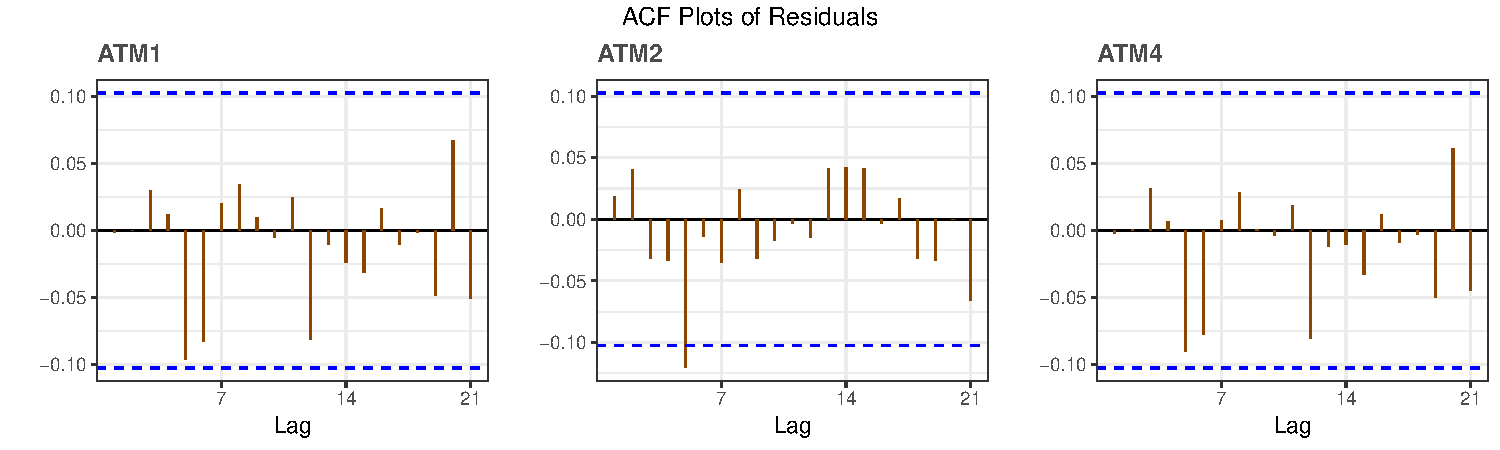
\includegraphics{Group2_Project1_Fall2019_files/figure-latex/unnamed-chunk-6-1.pdf}
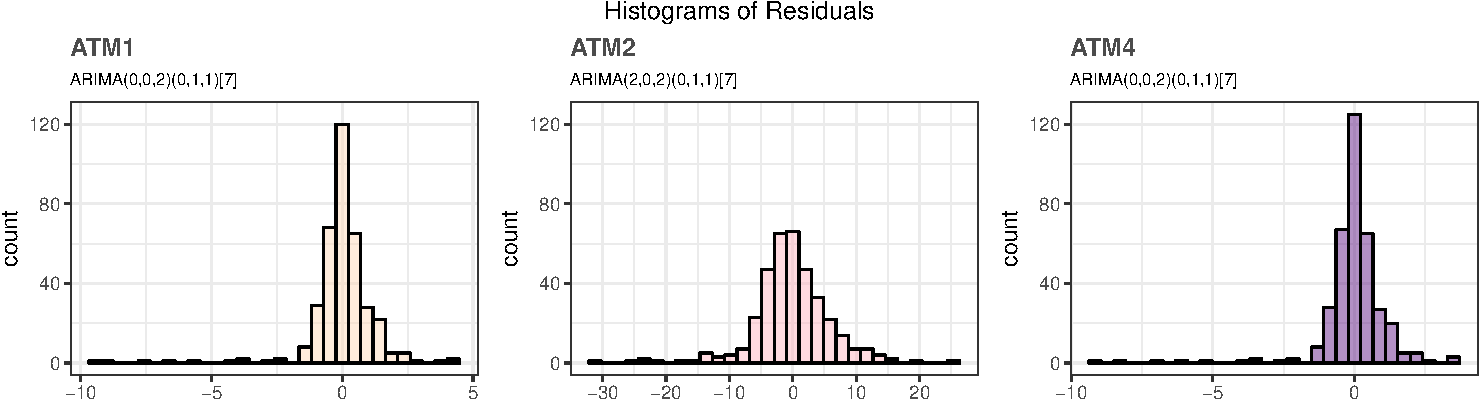
\includegraphics{Group2_Project1_Fall2019_files/figure-latex/unnamed-chunk-6-2.pdf}

\hypertarget{forecast}{%
\section{Forecast}\label{forecast}}

A forecast for the month of May will be 31 days in length. We applied a
forecast to each series, which spanned across 5 weeks. The numeric
forecasts can be viewed in a table output in the appendix section and
are also located within our data output folder.

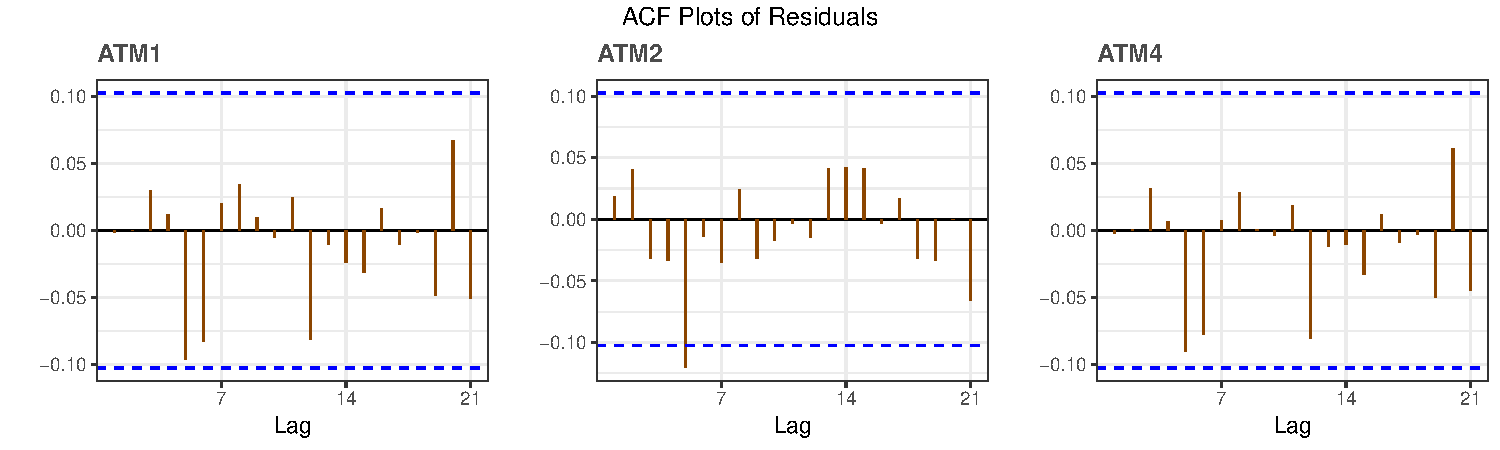
\includegraphics{Group2_Project1_Fall2019_files/figure-latex/unnamed-chunk-7-1.pdf}

\hypertarget{summary}{%
\section{Summary}\label{summary}}

Forecasts for ATM1, ATM2, and ATM4 reprise the clear, persistent weekly
pattern found in the historic data, with mid-week troughs and a largely
flat trend on a five-week time horizon. ATM1 and ATM4 experience sharper
troughs on Wednesdays; ATM2 drops on Tuesdays and bottoms out on
Wednesdays. Additionally, ATM2 has a slightly tighter confidence
interval than ATM1 and ATM4. The mean forecast for ATM3 based on three
data points is a useful estimate insofar as the assumptions it rests on
are sound: that the zero observations aren't measurement or data errors,
and that the three non-zero observations aren't outliers and in fact
convey information about a future pattern.

\hypertarget{part-b-forecasting-power}{%
\chapter{Part B: Forecasting Power}\label{part-b-forecasting-power}}

\begin{quote}
\textbf{Instructions:} Part B consists of a simple dataset of
residential power usage for January 1998 until December 2013. Your
assignment is to model these data and a monthly forecast for 2014. The
data is given in a single file. The variable `KWH' is power consumption
in Kilowatt hours, the rest is straight forward. Add these to your
existing files above - clearly labeled.
\end{quote}

\hypertarget{exploration-1}{%
\section{Exploration}\label{exploration-1}}

We observed a missing value in September 2008 and imputed it using
\texttt{na.interpolation}, which performs a technique in numerical
analysis to estimate a value from known data points (in our case, a
linear method using first order Taylor polynomials).

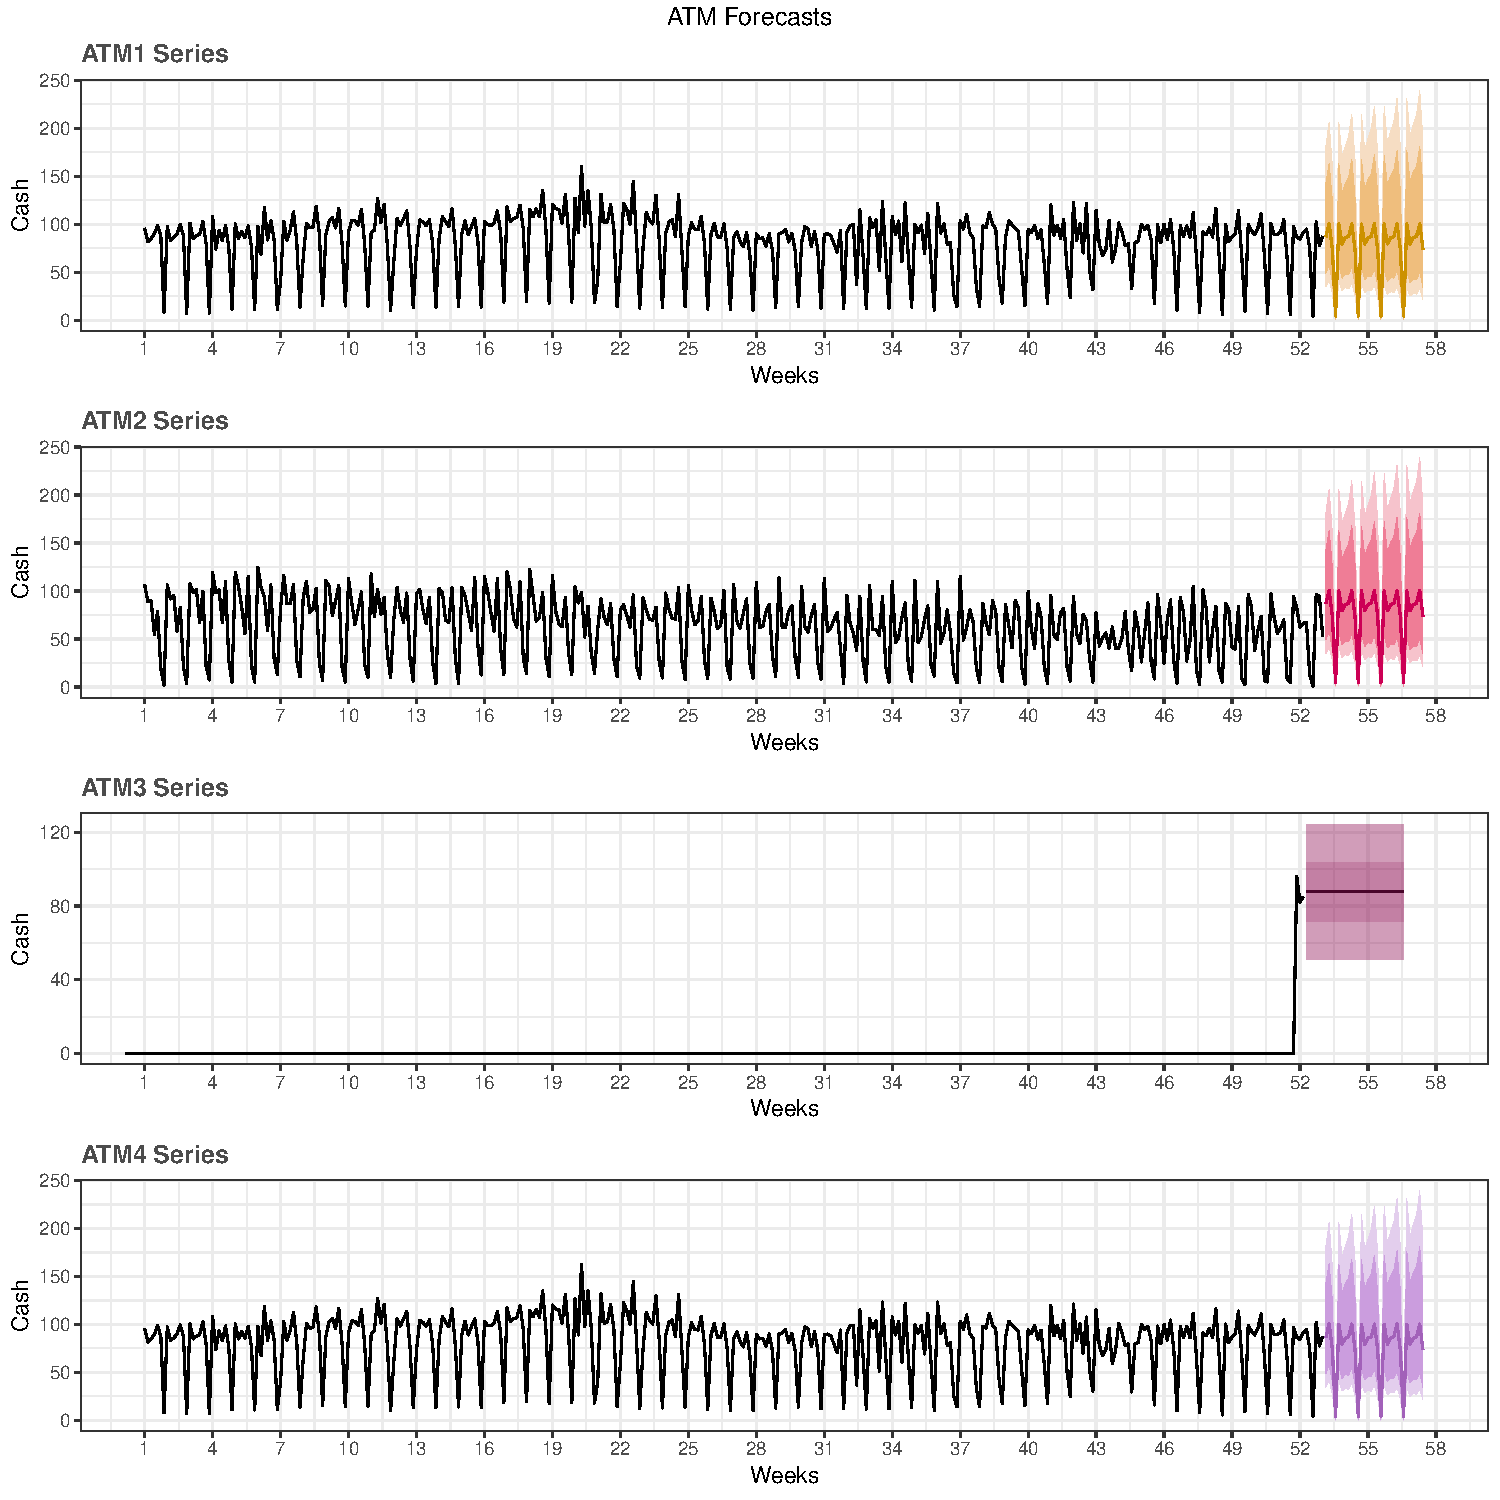
\includegraphics{Group2_Project1_Fall2019_files/figure-latex/unnamed-chunk-8-1.pdf}

Our time series plot reveals annual seasonality; box plots and
seasonality demonstrate where power consumption fluctuations occur
within each of the cycles. We speculate that this pattern could be due
to no major holidays that require power draining decor plus and minimal
air conditioning usage during cold months.

\hypertarget{evaluation-1}{%
\section{Evaluation}\label{evaluation-1}}

Power consumption increases between the months of June and August,
likely in relation to air conditioning usage. It dips from September to
Novemeber, followed by a small spike in December, which might be due the
holidays (perhaps even holiday lights).

Within the overall TS plot a dip in July 2010 is visible; this outlier
which may be the result of a power outtage during a hot summer month.
Using \texttt{TSOutliers}, we identify the outlier and replace it using
a Box-Cox transformation (by setting the lambda argument to automatic).

The ACF plot shows that autocorrelations are well outside the
significant space indicating the series is not white noise,
non-stationary.

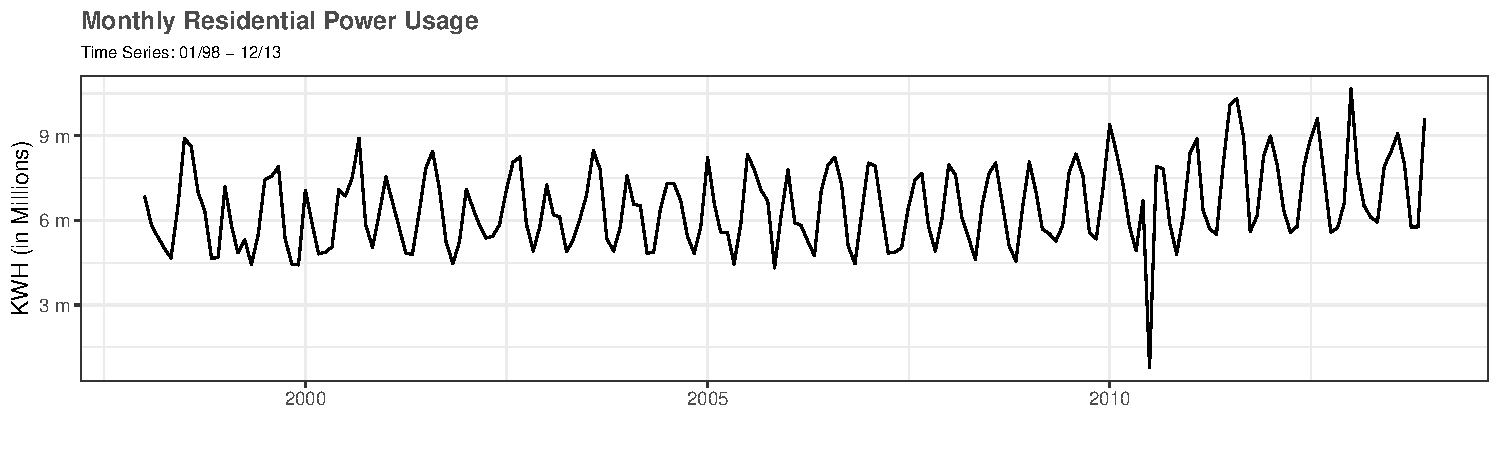
\includegraphics{Group2_Project1_Fall2019_files/figure-latex/unnamed-chunk-9-1.pdf}

\hypertarget{modeling-1}{%
\section{Modeling}\label{modeling-1}}

We built four different models using ARIMA, STL (with and without
dampening), and ETS methods. By checking residuals we can make some
preliminary observations on these models' reliability.

The residual ACF plots show residual autocorrelations for each of our
models. Model 1 (ARIMA) has less autocorrelation than the other three;
it is also well within the 95\% limits (indicated by dotted blue lines).

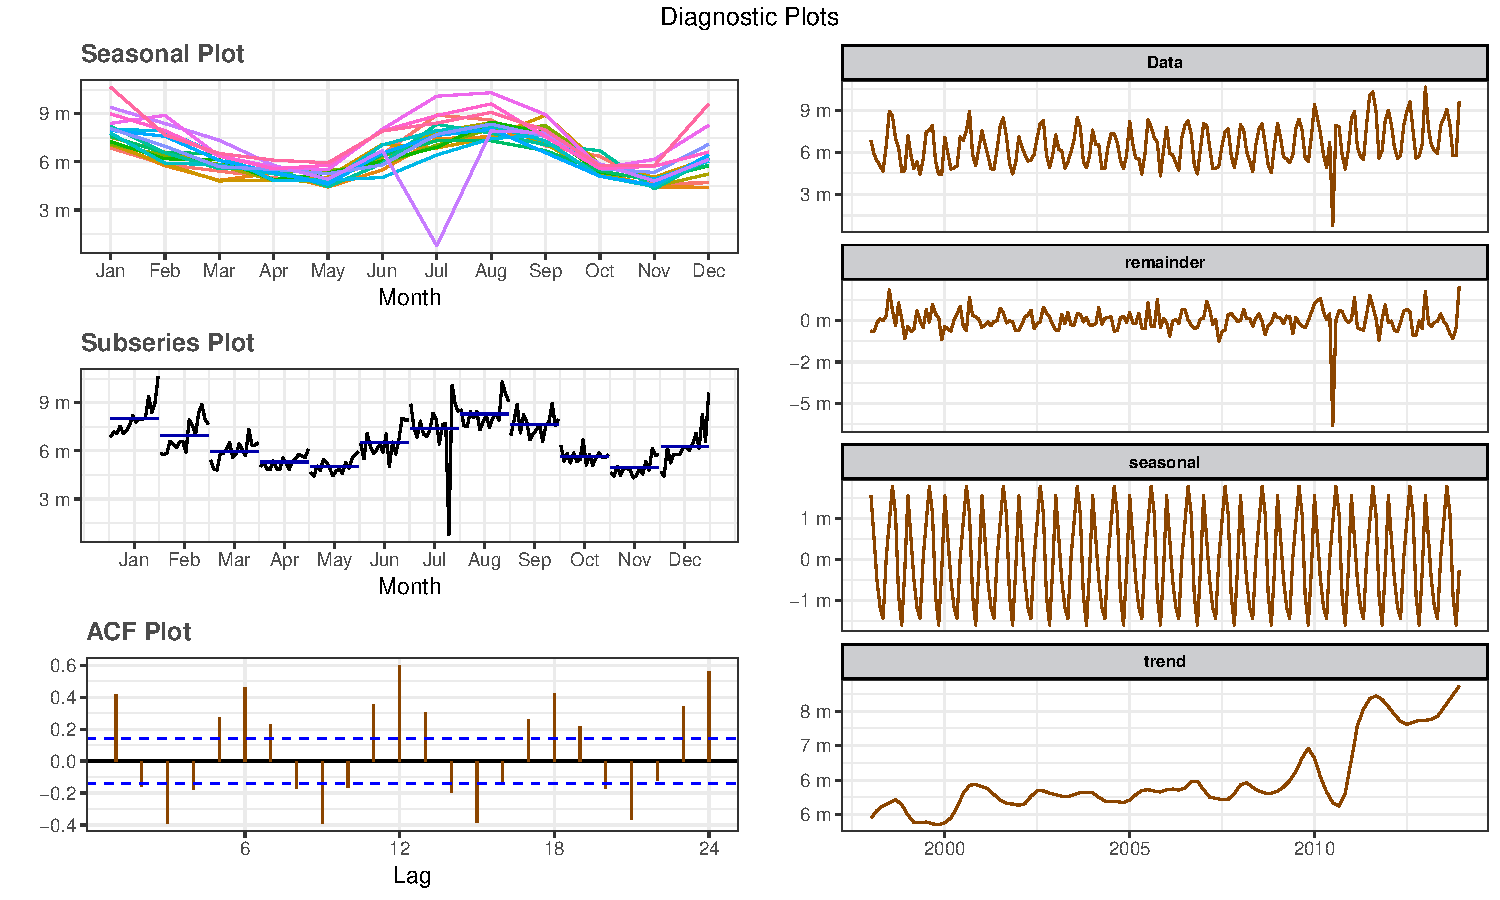
\includegraphics{Group2_Project1_Fall2019_files/figure-latex/unnamed-chunk-10-1.pdf}

The residuals for each of our models do not deviate substantially from
normality. While the residuals of Model 1 (ARIMA) do not have an
extended number of bins and this distorts the normality proximity, we
can regard the distribution as normal.

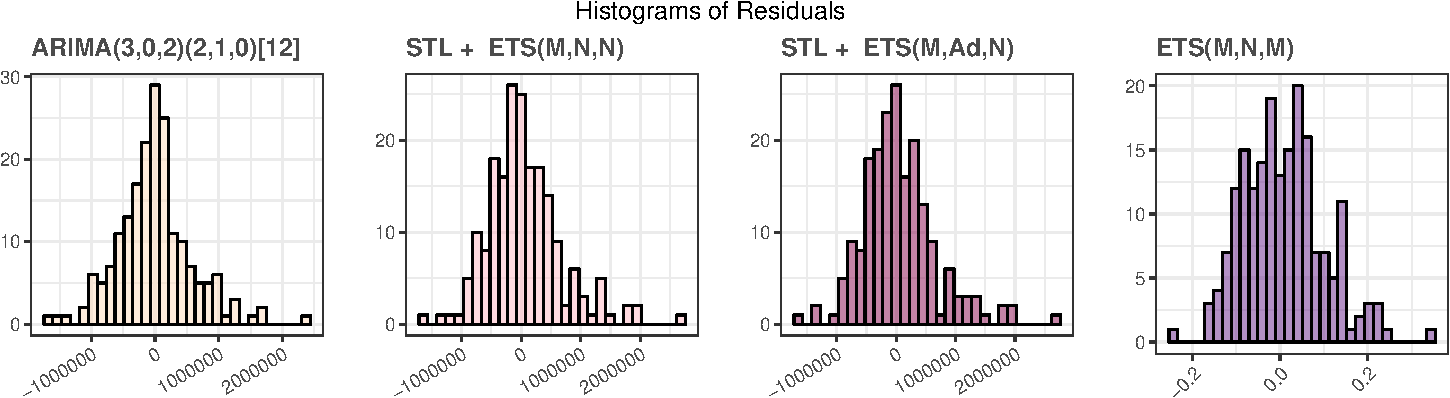
\includegraphics{Group2_Project1_Fall2019_files/figure-latex/unnamed-chunk-11-1.pdf}

A Ljung-Box test yields a p-value \textgreater{} 0.05 for Model 1
(ARIMA), implying that the residuals from other models are not
independent, hence not white noise. We will continue with this model for
forecasting; a full summary for this and other models attempted is
included in the appendix.

\hypertarget{forecast-1}{%
\section{Forecast}\label{forecast-1}}

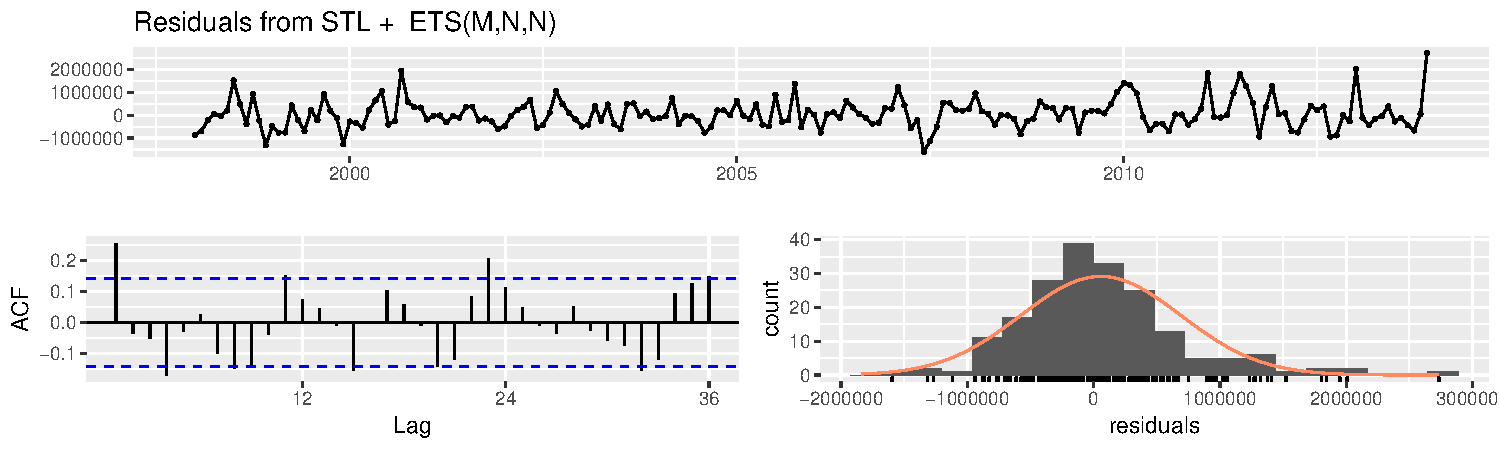
\includegraphics{Group2_Project1_Fall2019_files/figure-latex/unnamed-chunk-12-1.pdf}
The \texttt{auto.arima()} function performs cross validation on
hyperparameter tuning to find the best model with parameters of
\texttt{order} and \texttt{seasonal} that minimize \texttt{AIC}. This
approach yielded \textbf{arima\_model}: ARIMA\((3,0,2)(2,1,0)12\) with
drift resulting in an of \texttt{AIC} = 5332.24. As other models failed
the Ljung-Box test, we develop forecasts based only on the reliable
ARIMA model; forecasted values are included in the appendix.

\hypertarget{summary-1}{%
\section{Summary}\label{summary-1}}

We implemented a cross-validation method of testing for \texttt{h=12},
randomly choosing 12 points over the fitted model to measure and take
the average of RMSEs. By definition, a lower RMSE on test set indicates
a better forecast of the test data.

Using time series cross-validation, we compute RMSE on the test set
(\texttt{h=12}). If other models had not failed the Ljung-Box test, we
use the lowest RMSE as a criterion of selection. Cross-validation test
of the seasonal ARIMA model produces an RMSE on test set of around 720k,
and on training set of around 589k. We conclude the model is not
necessarily overfitted. This finding is consistent with the MAPE on the
training set that is less than 7.

\begin{verbatim}
[1] "RMSE - Train: 589381.7 ; RMSE - Test: 725175"
\end{verbatim}

\hypertarget{part-c-waterflow}{%
\chapter{Part C: Waterflow}\label{part-c-waterflow}}

\begin{quote}
\textbf{Instructions:} Part C consists of two data sets. These are
simple 2 columns sets, however they have different time stamps. Your
optional assignment is to time-base sequence the data and aggregate
based on hour (example of what this looks like, follows). Note for
multiple recordings within an hour, take the mean. Then to test
appropriate assumptions and forecast a week forward with confidence
bands (80 and 95\%). Add these to your existing files above - clearly
labeled.
\end{quote}

\hypertarget{exploration-2}{%
\section{Exploration}\label{exploration-2}}

Because of the disparities in the data some grooming was necessary:

\textbf{Pipe one:}\\
* 1000 observations * No missing values * Multiple reading within each
hour\\
* 9-days of data

\textbf{Pipe Two}\\
* 1000 Observations\\
* No missing values * Single reading on the hour * 41-days of data

Pipe One represents 9 days of water flow rate measurements with multiple
samples per hour. In order to align with hourly readings from Pipe Two,
a mean of all Pipe One rates in a given hour was taken and labeled by
its `floor' (i.e.~9 for mean of all times between 9:00 and 9:59
-inclusive of both bounds). After aggregating, this yielded 236
observations (spanning nine days) for Pipe One and 1000 observations
(spanning 41days) for Pipe Two.

The two data sets posed an interesting conundrum. We considered two
possible approaches:

\begin{enumerate}
\def\labelenumi{\arabic{enumi}.}
\tightlist
\item
  Merge the files and use only 236 observations.
\end{enumerate}

\begin{itemize}
\tightlist
\item
  All forecasts would be based on the combined data.
\item
  This would mean making 168 forecasts (\(7days x 24hours\)) with only
  236 data-points prior.
\item
  All forecasts would start November 1 rather than December 3 (the end
  of the most recent time series).\\
\end{itemize}

\begin{enumerate}
\def\labelenumi{\arabic{enumi}.}
\setcounter{enumi}{1}
\tightlist
\item
  Merge the files and use the whole set to make predictions.\\
\end{enumerate}

\begin{itemize}
\tightlist
\item
  We would have 1000 observations to model prior to forecasts.
\item
  236 of the observations would be be different from the remaining 764,
  which could both alter the model type and forecast.
\item
  We would forecast from the natural ending of the Pipe Two readings. In
  the end, it made the most sense to model the combined sets in their
  entireties, so method two was adopted.
\end{itemize}

Because daily periodicity is conceivable for this data, it was important
to use a frequency of 24 in converting this data. This entailed
numbering by day of year and grooming the time series to start on the
7081 hour (which aligns with October 23 01:00 AM our first merged
observation).

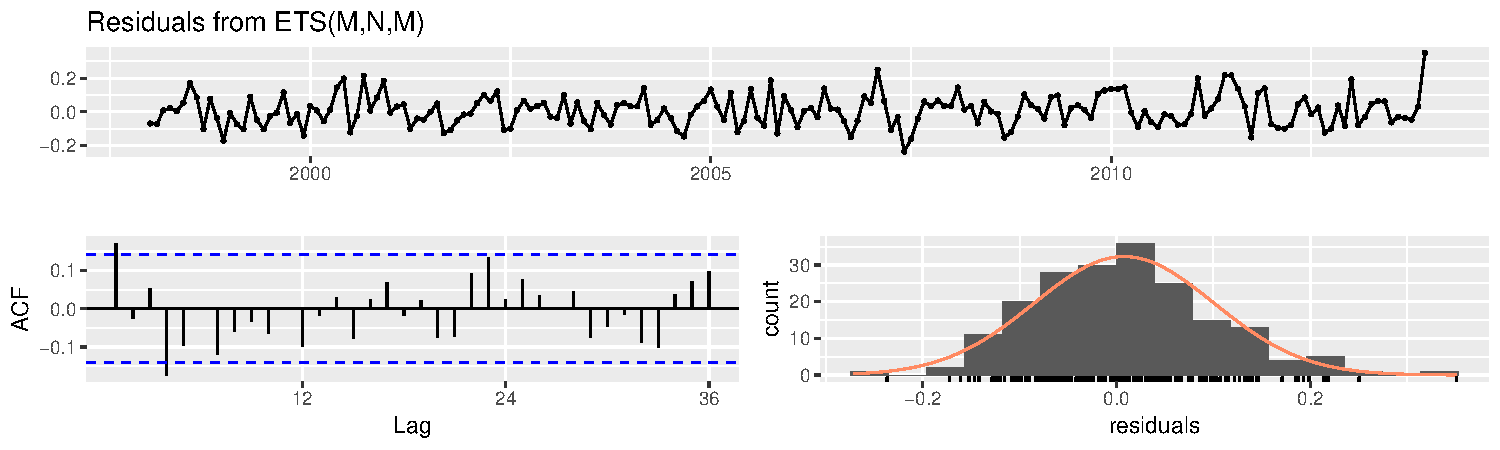
\includegraphics{Group2_Project1_Fall2019_files/figure-latex/unnamed-chunk-14-1.pdf}

\hypertarget{evaluation-2}{%
\section{Evaluation}\label{evaluation-2}}

\hypertarget{decomposition}{%
\subsection{Decomposition}\label{decomposition}}

It is clear from the combined plot that there is a pretty notable change
in the trend when the readings from Pipe One wane. We examined the
decomposed series for insight into a good model.

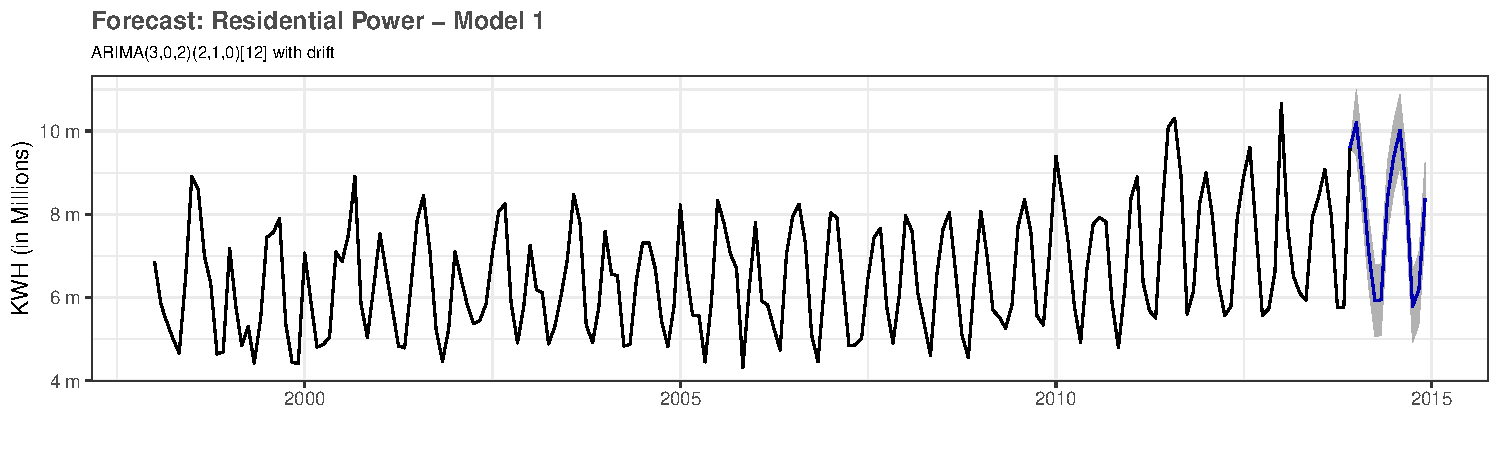
\includegraphics{Group2_Project1_Fall2019_files/figure-latex/unnamed-chunk-15-1.pdf}
From the decomposition, there appears to be a seasonal component, which
in agreement with the prior assessment that there might be a daily
flowrate periodicity. Also, as expected, around day 306, where Pipe One
flow rates go silent, there is a downward trend followed by a rolling
plateau thereafter.

\hypertarget{estimating-stationarity}{%
\subsection{Estimating Stationarity}\label{estimating-stationarity}}

Number of Estimated Differences using \texttt{ndiff()}: 1

\begin{verbatim}

    Augmented Dickey-Fuller Test

data:  ws
Dickey-Fuller = -6.4409, Lag order = 9, p-value = 0.01
alternative hypothesis: stationary
\end{verbatim}

Here we encounter contradictory estimates: \texttt{ndiffs()} suggests a
difference of 1, and the augmented dicky fuller test suggests that we
are stationary as-is. An \texttt{auto.arima()} may provide insight into
a reasonable starting place.

\hypertarget{estimating-orders-for-arima}{%
\subsection{Estimating Orders for
ARIMA}\label{estimating-orders-for-arima}}

\hypertarget{interpreting-the-acf-and-pacf}{%
\subsubsection{Interpreting the ACF and
PACF}\label{interpreting-the-acf-and-pacf}}

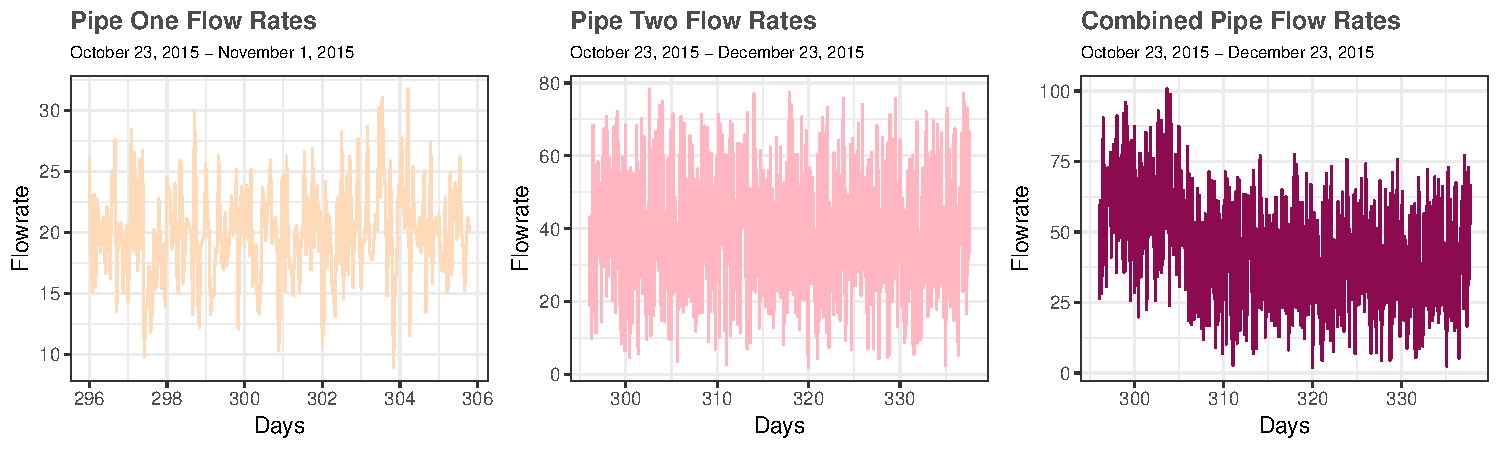
\includegraphics{Group2_Project1_Fall2019_files/figure-latex/unnamed-chunk-17-1.pdf}

As the ACF remains wholly above the critical threshold the series will
likely require differencing as suggested by the \texttt{ndiffs()}. There
is a spike at 24 on both PACF and ACF suggesting a daily period or
season that needs to be accounted for in our forecast.

\hypertarget{differenced-acf}{%
\subsubsection{Differenced ACF}\label{differenced-acf}}

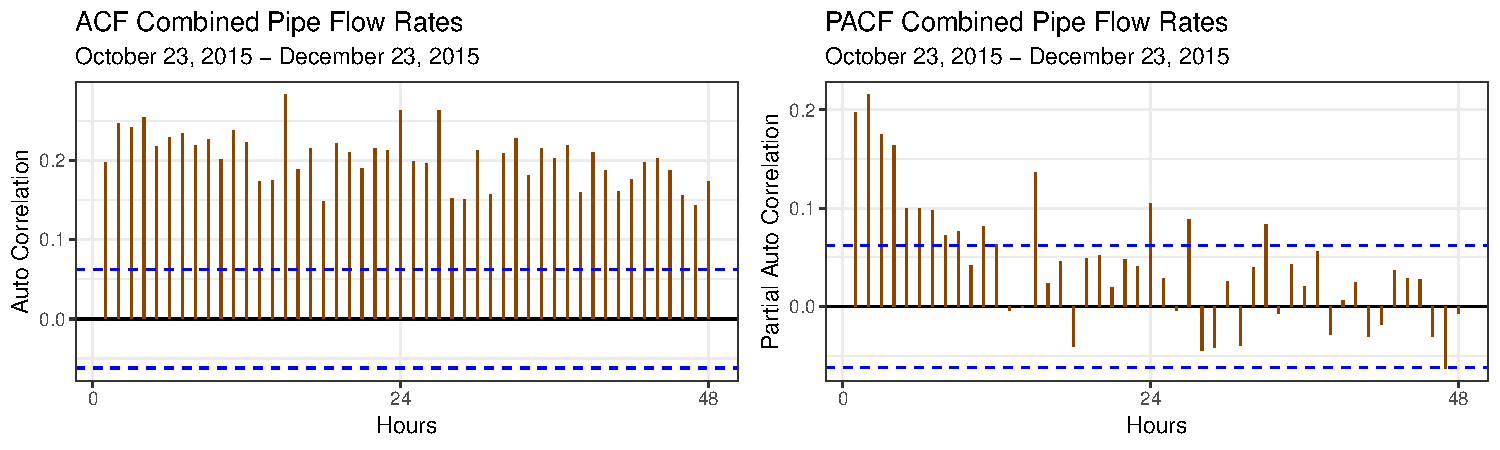
\includegraphics{Group2_Project1_Fall2019_files/figure-latex/unnamed-chunk-18-1.pdf}

We examined a final ACF of the differenced data to ensure that a second
first-order difference was not needed; while we assume \(d = 1\), the
appropriate value of \(q\) is not so clear, and seasonal orders were in
question, so we use \texttt{auto.arima()} to help iterate up on the best
starting place.

\hypertarget{modeling-2}{%
\section{Modeling}\label{modeling-2}}

The \texttt{auto.arima()} function was used in model selection. Using a
Box-Cox lambda value to normalize the data yields a
\(\lambda= .931552\). Because models can vary a lot based on the
selection criterion, both BIC and AIC models were run using lambda to
estimate a good starting place. We included the transformations in the
model (as opposed to outside the model) because we are using the ARIMA
function to difference the data automatically for more consistency and
flexibility in testing other model orders.

The \emph{AICc} chose a seasonal ARIMA of the following order:

\(ARIMA(1,1,3)(0,0,1)[24]\) \emph{AIC=7359.84 AICc=7359.9 BIC=7384.38}

The \emph{BIC} chose a non-seasonal ARIMA model as follows:

\(ARIMA(2,1,1)\) \emph{AIC=8082.22 AICc=8082.26 BIC=8101.85}

In both cases, the \texttt{auto.arima()} estimated that there needed to
be differencingm, which was supported by \texttt{ndiffs()} and our ACF
and PACF plots.

While both models' forecasts degrade pretty quickly towards the series
mean, the AICc model generates forecast that consider the variation
better before it levels out. Accordingly, we decided to explore and
attempt to tune this model to provide more robust predictions.

\textbf{AIC \(ARIMA(1,1,3)(0,0,1)[24]\) Residual Plots}

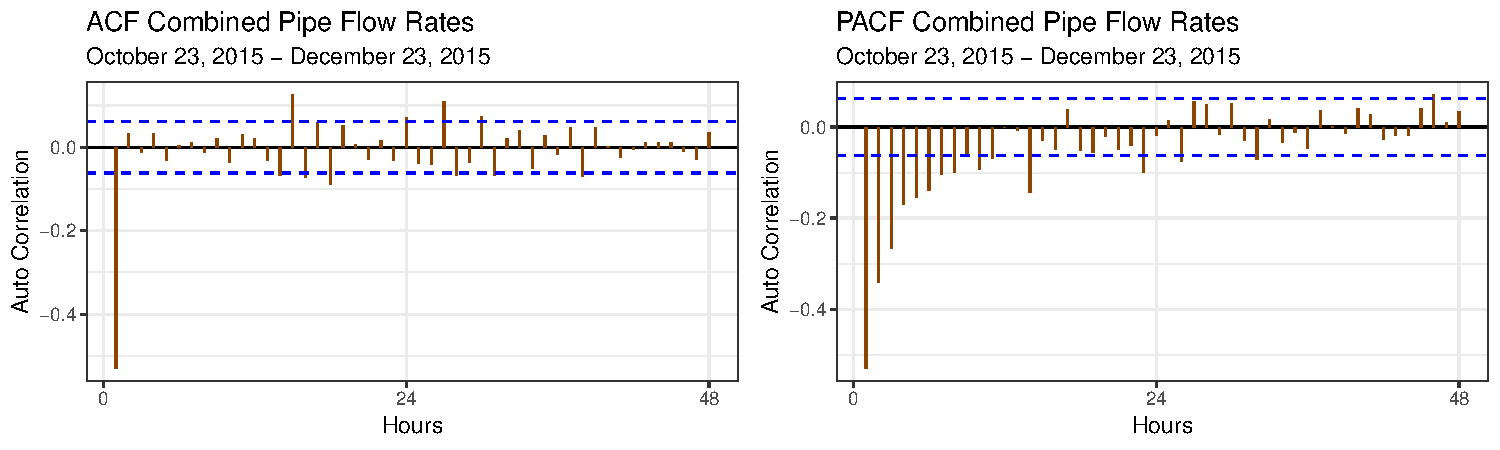
\includegraphics{Group2_Project1_Fall2019_files/figure-latex/unnamed-chunk-19-1.pdf}

\begin{verbatim}

    Ljung-Box test

data:  Residuals from ARIMA(1,1,3)(0,0,1)[24]
Q* = 57.362, df = 43, p-value = 0.07027

Model df: 5.   Total lags used: 48
\end{verbatim}

\textbf{BIC \(ARIMA(2,1,1)\) Residual Plots}

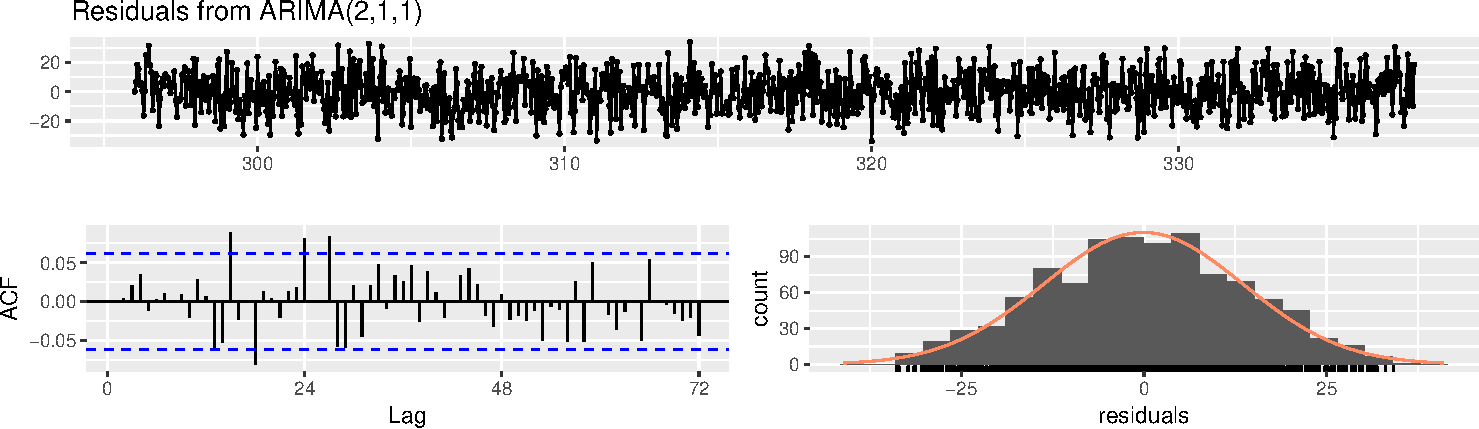
\includegraphics{Group2_Project1_Fall2019_files/figure-latex/unnamed-chunk-20-1.pdf}

\begin{verbatim}

    Ljung-Box test

data:  Residuals from ARIMA(2,1,1)
Q* = 64.403, df = 45, p-value = 0.03029

Model df: 3.   Total lags used: 48
\end{verbatim}

\hypertarget{interpreting-auto.arima}{%
\subsection{\texorpdfstring{Interpreting
\texttt{auto.arima()}}{Interpreting auto.arima()}}\label{interpreting-auto.arima}}

Both the AICc and BIC ARIMA models appear relatively `white-noisy', with
no autocorrelation on the first and 24th observations as well as
relatively normal residuals. However, examining the Ljung-Box test for
independence made clear that the Seasonal \(ARIMA (1,1,3)(0,0,1)[24]\)
is independent while the \(ARIMA(2,1,1)\) is not. This confirmed our
suspicion of unaccounted for seasonal variation in the model, which
required a seasonal MA(1) to rectify. To ensure that the best model had
been found, we varied p, q, and Q to determine if slight modifications
could improve the performance of the model.

\hypertarget{manual-arima-testing}{%
\subsection{Manual ARIMA testing}\label{manual-arima-testing}}

\begin{verbatim}
Series: ws 
ARIMA(1,1,3)(0,0,1)[24] 
Box Cox transformation: lambda= 0.9531552 

Coefficients:
         ar1      ma1     ma2      ma3    sma1
      0.7602  -1.7578  0.8286  -0.0614  0.0833
s.e.  0.1857   0.1874  0.1886   0.0324  0.0320

sigma^2 estimated as 187:  log likelihood=-4033.28
AIC=8078.56   AICc=8078.64   BIC=8108
\end{verbatim}

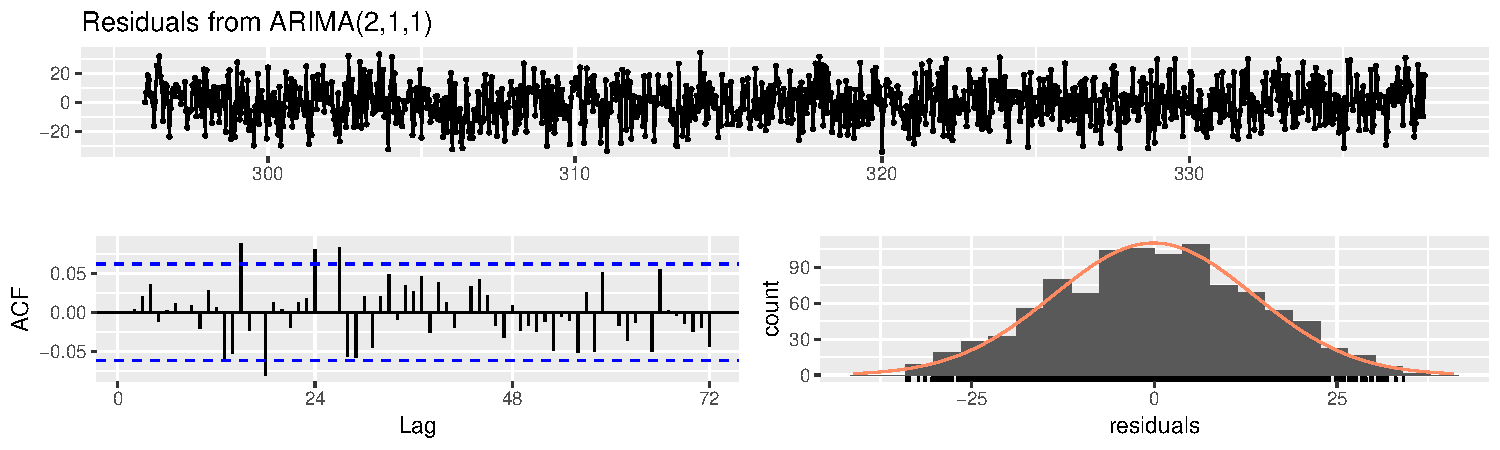
\includegraphics{Group2_Project1_Fall2019_files/figure-latex/unnamed-chunk-21-1.pdf}

\begin{verbatim}

    Ljung-Box test

data:  Residuals from ARIMA(1,1,3)(0,0,1)[24]
Q* = 47.142, df = 31, p-value = 0.03174

Model df: 5.   Total lags used: 36
\end{verbatim}

\hypertarget{forecast-2}{%
\section{Forecast}\label{forecast-2}}

\hypertarget{arima11300124}{%
\subsection{\texorpdfstring{\(ARIMA(1,1,3)(0,0,1)[24]\)}{ARIMA(1,1,3)(0,0,1){[}24{]}}}\label{arima11300124}}

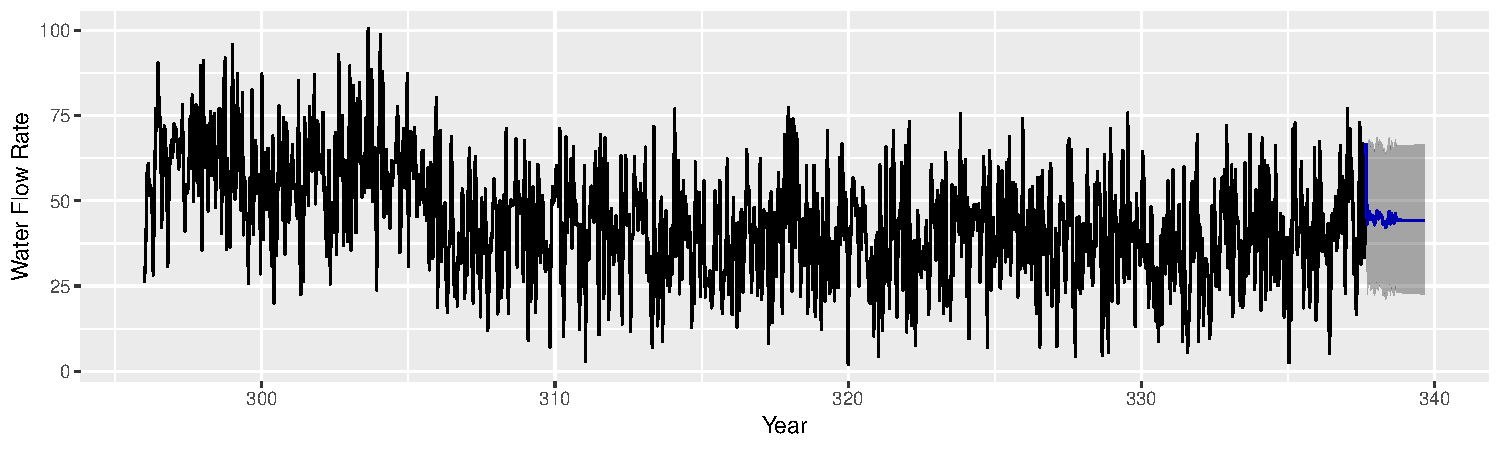
\includegraphics{Group2_Project1_Fall2019_files/figure-latex/unnamed-chunk-22-1.pdf}

\hypertarget{arima21300124}{%
\subsection{\texorpdfstring{\(ARIMA(2,1,3)(0,0,1)[24]\)}{ARIMA(2,1,3)(0,0,1){[}24{]}}}\label{arima21300124}}

\begin{verbatim}
Series: ws 
ARIMA(2,1,3)(0,0,1)[24] 
Box Cox transformation: lambda= 0.9531552 

Coefficients:
          ar1     ar2      ma1      ma2     ma3    sma1
      -0.1435  0.1884  -0.8478  -0.2709  0.1621  0.0798
s.e.      NaN  0.5408      NaN   0.6070  0.5319  0.0318

sigma^2 estimated as 187.5:  log likelihood=-4034.02
AIC=8082.05   AICc=8082.16   BIC=8116.4
\end{verbatim}

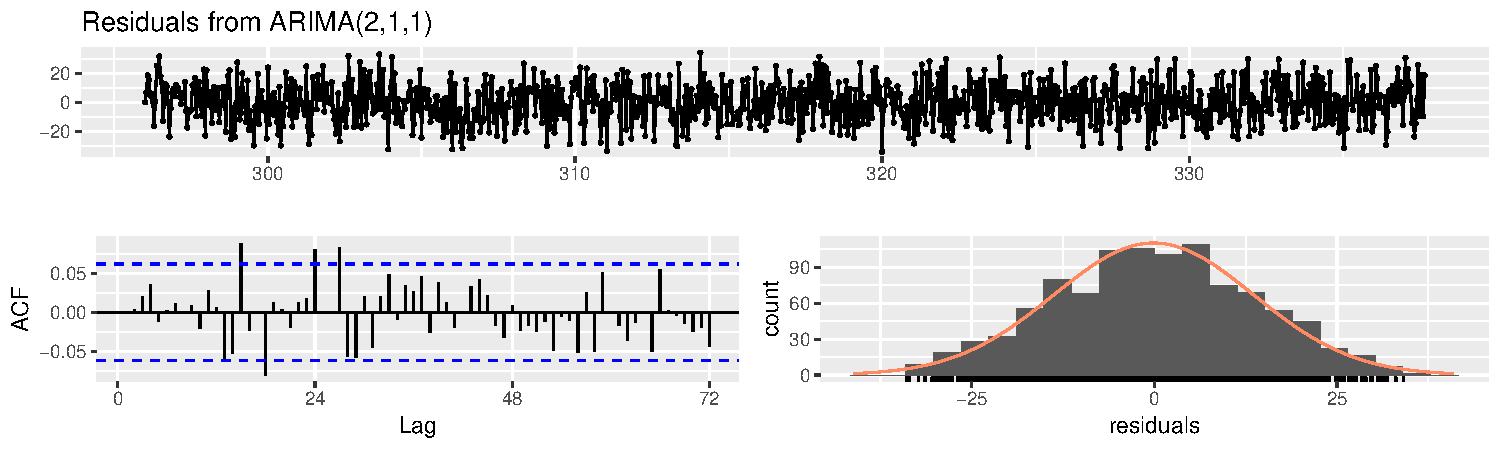
\includegraphics{Group2_Project1_Fall2019_files/figure-latex/unnamed-chunk-23-1.pdf}

\begin{verbatim}

    Ljung-Box test

data:  Residuals from ARIMA(2,1,3)(0,0,1)[24]
Q* = 48.506, df = 30, p-value = 0.01764

Model df: 6.   Total lags used: 36
\end{verbatim}

This Ljung-Box test shows unexplained variances in the residuals,
indicating that this model is not yet fully realized and inferior to the
Seasonal \(ARIMA (1,1,3)(0,0,1)[24]\).

\begin{verbatim}
Series: ws 
ARIMA(1,1,2)(0,0,1)[24] 
Box Cox transformation: lambda= 0.9531552 

Coefficients:
          ar1      ma1      ma2    sma1
      -0.2655  -0.7307  -0.2103  0.0790
s.e.   0.9490   0.9533   0.9121  0.0318

sigma^2 estimated as 187.1:  log likelihood=-4034.08
AIC=8078.16   AICc=8078.22   BIC=8102.7
\end{verbatim}

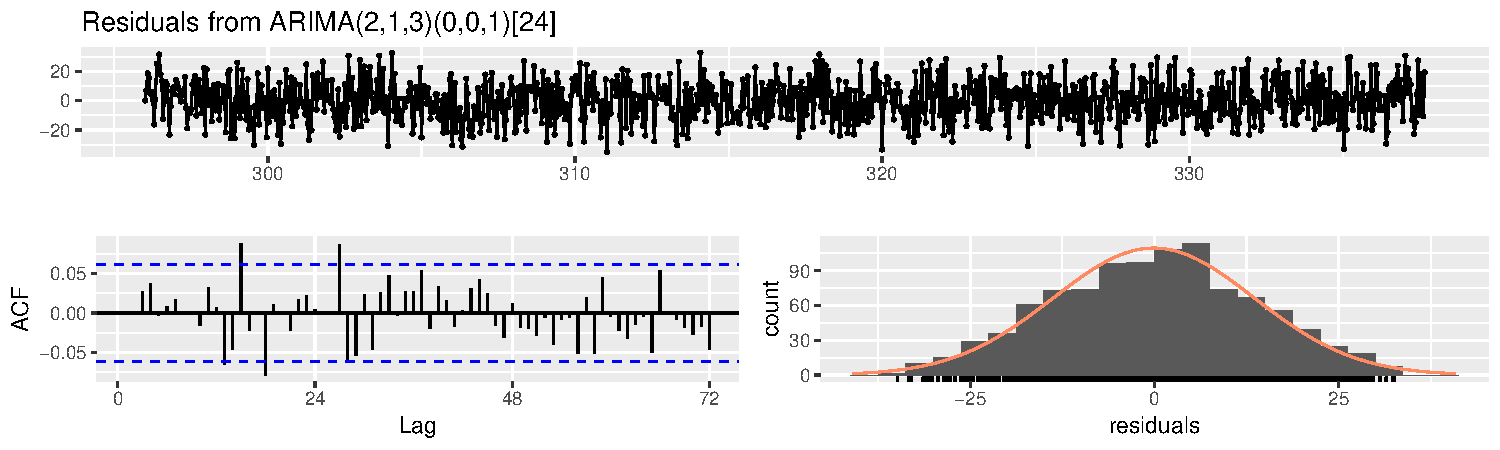
\includegraphics{Group2_Project1_Fall2019_files/figure-latex/unnamed-chunk-24-1.pdf}

\begin{verbatim}

    Ljung-Box test

data:  Residuals from ARIMA(1,1,2)(0,0,1)[24]
Q* = 47.963, df = 32, p-value = 0.03467

Model df: 4.   Total lags used: 36
\end{verbatim}

This Ljung-Box also shows unexplained variances in the residuals,
indicating that this model is not yet fully realized and inferior to the
Seasonal \(ARIMA (1,1,2)(0,0,1)[24]\).

\begin{verbatim}
Series: ws 
ARIMA(1,1,3) 
Box Cox transformation: lambda= 0.9531552 

Coefficients:
         ar1      ma1     ma2      ma3
      0.6792  -1.6742  0.7437  -0.0553
s.e.  0.2923   0.2930  0.2903   0.0330

sigma^2 estimated as 188.1:  log likelihood=-4036.63
AIC=8083.27   AICc=8083.33   BIC=8107.81
\end{verbatim}

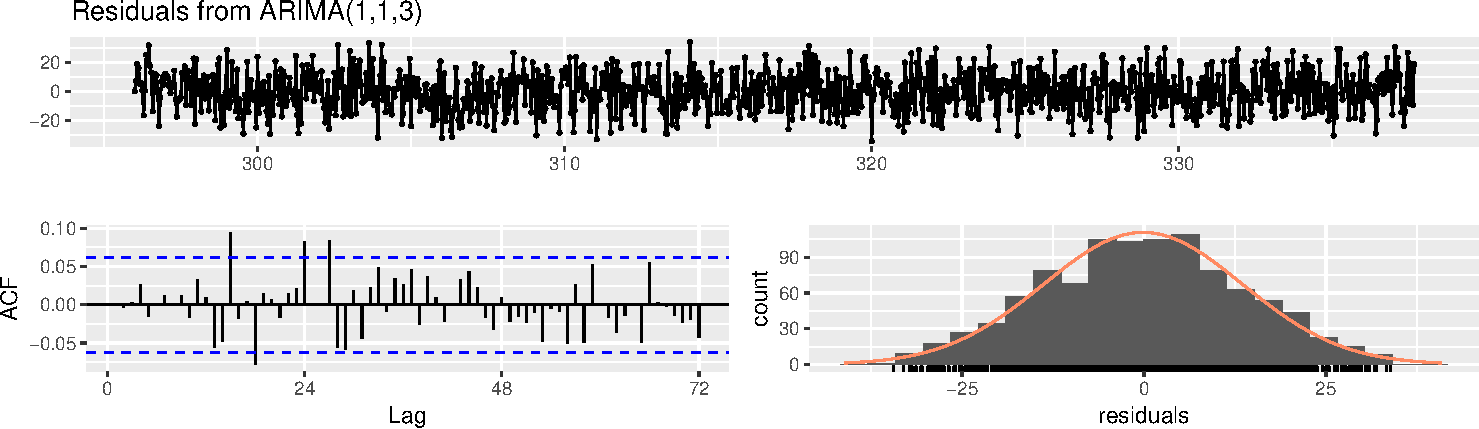
\includegraphics{Group2_Project1_Fall2019_files/figure-latex/unnamed-chunk-25-1.pdf}

\begin{verbatim}

    Ljung-Box test

data:  Residuals from ARIMA(1,1,3)
Q* = 53.61, df = 32, p-value = 0.009708

Model df: 4.   Total lags used: 36
\end{verbatim}

This Ljung-Box also shows unexplained variances in the residuals,
indicating that this model is not yet fully realized and inferior to the
Seasonal \(ARIMA (1,1,3)\).

\hypertarget{accepting-the-auto.arima}{%
\subsection{\texorpdfstring{Accepting the
\texttt{auto.arima()}}{Accepting the auto.arima()}}\label{accepting-the-auto.arima}}

Given that the other models show unexplained variance in the residuals,
we made our final predictions using the AICc recommended model of
\(ARIMA (1,1,3)(0,0,1)[24]\).

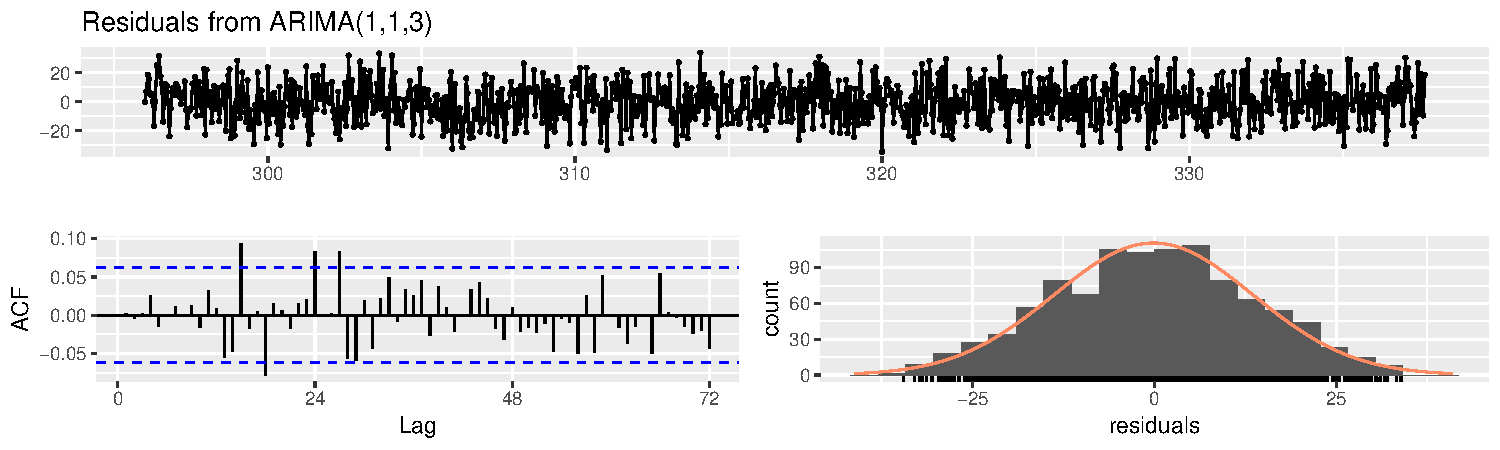
\includegraphics{Group2_Project1_Fall2019_files/figure-latex/unnamed-chunk-26-1.pdf}

\hypertarget{forecast-accuracy}{%
\subsection{Forecast Accuracy}\label{forecast-accuracy}}

\begin{tabular}{l|r|r|r|r|r|r|r}
\hline
  & ME & RMSE & MAE & MPE & MAPE & MASE & ACF1\\
\hline
Training set & 0.0015679 & 16.27402 & 13.23093 & -28.76247 & 50.34448 & 0.7489308 & 0.0014339\\
\hline
\end{tabular}

\hypertarget{summary-2}{%
\section{Summary}\label{summary-2}}

Ultimately, we assess that the Seasonal \(ARIMA (1,1,3)\) model is
marginally useful given its Mean Absolute Percentage of Error. This
measure indicates that on average each forecast differs from the actual
value on percentage basis by around 50\%. As is visible in the above
graph, which depicts the last 150 points in the time series as well as
our forecasts, predictions modulate around the mean and deteriorate to
it pretty quickly.

The original decomposition revelaed very little trend, a lot of
seasonality, and a substatial amount of random noise. The extensive
random noise component, is assumed to be responsible for the majority of
the error, as white noise is never predictable.

\hypertarget{appendix-a}{%
\chapter*{Appendix A}\label{appendix-a}}
\addcontentsline{toc}{chapter}{Appendix A}

\hypertarget{summary-a}{%
\subsection*{Summary Statistics}\label{summary-a}}
\addcontentsline{toc}{subsection}{Summary Statistics}

\begin{longtable}[]{@{}lrrrrrrrrrrrr@{}}
\toprule
ATM & n & mean & sd & median & trimmed & mad & min & max & range & skew
& kurtosis & se\tabularnewline
\midrule
\endhead
ATM1 & 365 & 84.10 & 36.60 & 91.0 & 86.86 & 25.20 & 1 & 180 & 179 &
-0.72 & 0.21 & 1.92\tabularnewline
ATM2 & 364 & 62.46 & 38.90 & 66.5 & 62.09 & 49.67 & 0 & 147 & 147 &
-0.03 & -1.10 & 2.04\tabularnewline
ATM3 & 365 & 0.72 & 7.94 & 0.0 & 0.00 & 0.00 & 0 & 96 & 96 & 10.93 &
118.38 & 0.42\tabularnewline
ATM4 & 365 & 86.84 & 65.52 & 91.0 & 86.86 & 25.20 & 1 & 1123 & 1122 &
10.67 & 168.66 & 3.43\tabularnewline
\bottomrule
\end{longtable}

\hypertarget{arima-a}{%
\subsection*{ARIMA Model Summary}\label{arima-a}}
\addcontentsline{toc}{subsection}{ARIMA Model Summary}

\textbf{\texttt{ATM1}:}

\begin{verbatim}
Series: ATM1_ts 
ARIMA(0,0,2)(0,1,1)[7] 
Box Cox transformation: lambda= 0.2584338 

Coefficients:
         ma1      ma2     sma1
      0.1085  -0.1089  -0.6425
s.e.  0.0524   0.0521   0.0431

sigma^2 estimated as 1.726:  log likelihood=-606.1
AIC=1220.2   AICc=1220.32   BIC=1235.72
\end{verbatim}

\textbf{\texttt{ATM2}:}

\begin{verbatim}
Series: ATM2_ts 
ARIMA(2,0,2)(0,1,1)[7] 
Box Cox transformation: lambda= 0.661752 

Coefficients:
          ar1      ar2     ma1     ma2     sma1
      -0.4238  -0.8978  0.4766  0.7875  -0.7064
s.e.   0.0592   0.0473  0.0883  0.0608   0.0417

sigma^2 estimated as 38.94:  log likelihood=-1162.96
AIC=2337.93   AICc=2338.17   BIC=2361.21
\end{verbatim}

\textbf{\texttt{ATM4}:}

\begin{verbatim}
Series: ATM4_ts 
ARIMA(0,0,2)(0,1,1)[7] 
Box Cox transformation: lambda= 0.2328582 

Coefficients:
         ma1      ma2     sma1
      0.1095  -0.1088  -0.6474
s.e.  0.0524   0.0523   0.0420

sigma^2 estimated as 1.439:  log likelihood=-573.5
AIC=1154.99   AICc=1155.11   BIC=1170.52
\end{verbatim}

\hypertarget{forecast-a}{%
\subsection*{Point Forecasts}\label{forecast-a}}
\addcontentsline{toc}{subsection}{Point Forecasts}

\begin{table}[H]

\caption{\label{tab:unnamed-chunk-31}ATM Mean Point Forecast}
\centering
\begin{tabu} to \linewidth {>{\raggedright}X>{\raggedleft}X>{\raggedleft}X>{\raggedleft}X>{\raggedleft}X}
\hline
\textbf{Date} & \textbf{ATM1} & \textbf{ATM2} & \textbf{ATM3} & \textbf{ATM4}\\
\hline
\rowcolor{gray!6}  2010-05-01 & 87 & 66 & 88 & 87\\
\hline
2010-05-02 & 101 & 71 & 88 & 101\\
\hline
\rowcolor{gray!6}  2010-05-03 & 74 & 11 & 88 & 74\\
\hline
2010-05-04 & 4 & 2 & 88 & 4\\
\hline
\rowcolor{gray!6}  2010-05-05 & 100 & 98 & 88 & 100\\
\hline
2010-05-06 & 79 & 89 & 88 & 79\\
\hline
\rowcolor{gray!6}  2010-05-07 & 86 & 66 & 88 & 86\\
\hline
2010-05-08 & 87 & 66 & 88 & 87\\
\hline
\rowcolor{gray!6}  2010-05-09 & 100 & 71 & 88 & 100\\
\hline
2010-05-10 & 74 & 11 & 88 & 74\\
\hline
\rowcolor{gray!6}  2010-05-11 & 4 & 2 & 88 & 4\\
\hline
2010-05-12 & 100 & 98 & 88 & 100\\
\hline
\rowcolor{gray!6}  2010-05-13 & 79 & 89 & 88 & 79\\
\hline
2010-05-14 & 86 & 66 & 88 & 86\\
\hline
\rowcolor{gray!6}  2010-05-15 & 87 & 66 & 88 & 87\\
\hline
2010-05-16 & 100 & 71 & 88 & 100\\
\hline
\rowcolor{gray!6}  2010-05-17 & 74 & 11 & 88 & 74\\
\hline
2010-05-18 & 4 & 2 & 88 & 4\\
\hline
\rowcolor{gray!6}  2010-05-19 & 100 & 98 & 88 & 100\\
\hline
2010-05-20 & 79 & 89 & 88 & 79\\
\hline
\rowcolor{gray!6}  2010-05-21 & 86 & 66 & 88 & 86\\
\hline
2010-05-22 & 87 & 66 & 88 & 87\\
\hline
\rowcolor{gray!6}  2010-05-23 & 100 & 71 & 88 & 100\\
\hline
2010-05-24 & 74 & 11 & 88 & 74\\
\hline
\rowcolor{gray!6}  2010-05-25 & 4 & 2 & 88 & 4\\
\hline
2010-05-26 & 100 & 98 & 88 & 100\\
\hline
\rowcolor{gray!6}  2010-05-27 & 79 & 89 & 88 & 79\\
\hline
2010-05-28 & 86 & 66 & 88 & 86\\
\hline
\rowcolor{gray!6}  2010-05-29 & 87 & 66 & 88 & 87\\
\hline
2010-05-30 & 100 & 71 & 88 & 100\\
\hline
\rowcolor{gray!6}  2010-05-31 & 74 & 11 & 88 & 74\\
\hline
\end{tabu}
\end{table}

\newpage

\hypertarget{script-a}{%
\subsection*{R Script}\label{script-a}}
\addcontentsline{toc}{subsection}{R Script}

\begin{Shaded}
\begin{Highlighting}[]
\CommentTok{# Load data}
\NormalTok{atm_data <-}\StringTok{ }\KeywordTok{read_excel}\NormalTok{(}\StringTok{"data/ATM624Data.xlsx"}\NormalTok{) }

\CommentTok{# clean dataframe}
\NormalTok{atm <-}\StringTok{ }\NormalTok{atm_data }\OperatorTok\StringTok{ }
\StringTok{  }\CommentTok{# create wide dataframe}
\StringTok{  }\KeywordTok{spread}\NormalTok{(ATM, Cash) }\OperatorTok\StringTok{ }
\StringTok{  }\CommentTok{# remove NA column using function from janitor package}
\StringTok{  }\KeywordTok{remove_empty}\NormalTok{(}\DataTypeTok{which =} \StringTok{"cols"}\NormalTok{) }\OperatorTok
\StringTok{  }\CommentTok{# filter unobserved values from May 2010 }
\StringTok{  }\KeywordTok{filter}\NormalTok{(DATE }\OperatorTok{<}\StringTok{ }\KeywordTok{as.Date}\NormalTok{(}\StringTok{"2010-05-01"}\NormalTok{)) }\OperatorTok\StringTok{ }\KeywordTok{arrange}\NormalTok{(DATE) }

\NormalTok{atm}\OperatorTok{$}\NormalTok{ATM2[}\KeywordTok{is.na}\NormalTok{(atm}\OperatorTok{$}\NormalTok{ATM2)] <-}\StringTok{ }\KeywordTok{mean}\NormalTok{(atm}\OperatorTok{$}\NormalTok{ATM2, }\DataTypeTok{na.rm =} \OtherTok{TRUE}\NormalTok{) }\CommentTok{## remove NA}
\NormalTok{atm}\OperatorTok{$}\NormalTok{ATM4[}\KeywordTok{which.max}\NormalTok{(atm}\OperatorTok{$}\NormalTok{ATM4)] <-}\StringTok{ }\KeywordTok{mean}\NormalTok{(atm}\OperatorTok{$}\NormalTok{ATM4, }\DataTypeTok{na.rm =} \OtherTok{TRUE}\NormalTok{) }\CommentTok{## remove outlier}

\CommentTok{# create TS with weekly frequency & subset data}
\NormalTok{atm_ts <-}\StringTok{ }\NormalTok{atm }\OperatorTok\StringTok{ }\KeywordTok{select}\NormalTok{(}\OperatorTok{-}\NormalTok{DATE) }\OperatorTok\StringTok{ }\KeywordTok{ts}\NormalTok{(}\DataTypeTok{start=}\DecValTok{1}\NormalTok{,  }\DataTypeTok{frequency =} \DecValTok{7}\NormalTok{)}
\NormalTok{ATM1_ts <-}\StringTok{ }\NormalTok{atm_ts[,}\DecValTok{1}\NormalTok{]; ATM2_ts <-}\StringTok{ }\NormalTok{atm_ts[,}\DecValTok{2}\NormalTok{]; ATM3_ts <-}\StringTok{ }\NormalTok{atm_ts[,}\DecValTok{3}\NormalTok{]; ATM4_ts <-}\StringTok{ }\NormalTok{atm_ts[,}\DecValTok{4}\NormalTok{]}

\CommentTok{#unit root test: }
\NormalTok{ATM1_ur <-}\KeywordTok{ur.kpss}\NormalTok{(ATM1_ts); ATM2_ur <-}\KeywordTok{ur.kpss}\NormalTok{(ATM2_ts); ATM4_ur <-}\KeywordTok{ur.kpss}\NormalTok{(ATM4_ts)}
\NormalTok{ATM1d_ur <-}\KeywordTok{ur.kpss}\NormalTok{(}\KeywordTok{diff}\NormalTok{(ATM1_ts, }\DataTypeTok{lag=}\DecValTok{7}\NormalTok{)); ATM2d_ur <-}\KeywordTok{ur.kpss}\NormalTok{(}\KeywordTok{diff}\NormalTok{(ATM2_ts, }\DataTypeTok{lag=}\DecValTok{7}\NormalTok{))}
\NormalTok{ATM4d_ur <-}\KeywordTok{ur.kpss}\NormalTok{(}\KeywordTok{diff}\NormalTok{(ATM4_ts, }\DataTypeTok{lag=}\DecValTok{7}\NormalTok{))}

\CommentTok{# AUTO.ARIMA function; set D=1 for seasonal differencing}
\NormalTok{ATM1_AA <-}\KeywordTok{auto.arima}\NormalTok{(ATM1_ts, }\DataTypeTok{D =} \DecValTok{1}\NormalTok{, }\DataTypeTok{lambda =} \StringTok{"auto"}\NormalTok{, }\DataTypeTok{approximation =}\NormalTok{ F, }\DataTypeTok{stepwise =}\NormalTok{ T)}
\NormalTok{ATM2_AA <-}\KeywordTok{auto.arima}\NormalTok{(ATM2_ts, }\DataTypeTok{D =} \DecValTok{1}\NormalTok{, }\DataTypeTok{lambda =} \StringTok{"auto"}\NormalTok{, }\DataTypeTok{approximation =}\NormalTok{ F, }\DataTypeTok{stepwise =}\NormalTok{ T)}
\NormalTok{ATM4_AA <-}\KeywordTok{auto.arima}\NormalTok{(ATM4_ts, }\DataTypeTok{D =} \DecValTok{1}\NormalTok{, }\DataTypeTok{lambda =} \StringTok{"auto"}\NormalTok{, }\DataTypeTok{approximation =}\NormalTok{ F, }\DataTypeTok{stepwise =}\NormalTok{ T)}

\CommentTok{# Forecast Results}
\NormalTok{ATM1_fc <-}\StringTok{ }\KeywordTok{forecast}\NormalTok{(ATM1_AA,}\DataTypeTok{h=}\DecValTok{31}\NormalTok{); ATM2_fc <-}\StringTok{ }\KeywordTok{forecast}\NormalTok{(ATM2_AA,}\DataTypeTok{h=}\DecValTok{31}\NormalTok{)}
\NormalTok{ATM3_fc <-}\StringTok{ }\KeywordTok{meanf}\NormalTok{(ATM3_ts[ATM3_ts }\OperatorTok{>}\StringTok{ }\DecValTok{0}\NormalTok{], }\DataTypeTok{h=}\DecValTok{31}\NormalTok{); ATM4_fc <-}\StringTok{ }\KeywordTok{forecast}\NormalTok{(ATM4_AA,}\DataTypeTok{h=}\DecValTok{31}\NormalTok{)}

\CommentTok{# Prepare dataframe for ATM3 mean forcast plotting }
\NormalTok{ATM3_plotdata_fc <-}\StringTok{ }\KeywordTok{cbind}\NormalTok{(}\KeywordTok{seq}\NormalTok{(}\DataTypeTok{from =} \DecValTok{366}\NormalTok{, }\DataTypeTok{to =} \DecValTok{396}\NormalTok{), ATM3_fc[[}\DecValTok{5}\NormalTok{]], ATM3_fc[[}\DecValTok{6}\NormalTok{]], }
\NormalTok{                          ATM3_fc[[}\DecValTok{7}\NormalTok{]]) }\OperatorTok\StringTok{ }\KeywordTok{as.data.frame}\NormalTok{()}

\KeywordTok{colnames}\NormalTok{(ATM3_plotdata_fc) <-}\StringTok{ }\KeywordTok{c}\NormalTok{(}\StringTok{'Date'}\NormalTok{, }\StringTok{'Point Forecast'}\NormalTok{, }
                                \StringTok{'Lo 80'}\NormalTok{, }\StringTok{'Lo 95'}\NormalTok{, }\StringTok{'Hi 80'}\NormalTok{, }\StringTok{'Hi 95'}\NormalTok{)}
\NormalTok{ATM3_plotdata <-}\StringTok{ }\NormalTok{ATM3_ts }\OperatorTok\StringTok{ }\KeywordTok{fortify}\NormalTok{() }\OperatorTok\StringTok{ }\KeywordTok{select}\NormalTok{(}\OperatorTok{-}\NormalTok{Index) }\OperatorTok\StringTok{ }\KeywordTok{rename}\NormalTok{(}\DataTypeTok{Cash =}\NormalTok{ Data) }\OperatorTok\StringTok{ }
\StringTok{  }\KeywordTok{mutate}\NormalTok{(}\DataTypeTok{Date =} \KeywordTok{as.numeric}\NormalTok{(}\KeywordTok{row.names}\NormalTok{(.))) }\OperatorTok\StringTok{ }\KeywordTok{select}\NormalTok{(Date, Cash) }\OperatorTok\StringTok{ }
\StringTok{  }\KeywordTok{full_join}\NormalTok{(ATM3_plotdata_fc, }\DataTypeTok{by =} \StringTok{'Date'}\NormalTok{)}

\CommentTok{#Revert results back into original form}
\NormalTok{date <-}\StringTok{ }\KeywordTok{as.character}\NormalTok{(}\KeywordTok{seq}\NormalTok{(}\KeywordTok{as.Date}\NormalTok{(}\StringTok{'2010-05-01'}\NormalTok{), }\DataTypeTok{length.out=}\DecValTok{31}\NormalTok{, }\DataTypeTok{by=}\DecValTok{1}\NormalTok{))}
\NormalTok{ATM_FC <-}\StringTok{  }\KeywordTok{cbind}\NormalTok{(}\StringTok{"Date"}\NormalTok{=date, }\StringTok{"ATM1"}\NormalTok{=ATM1_fc}\OperatorTok{$}\NormalTok{mean, }\StringTok{"ATM2"}\NormalTok{=ATM2_fc}\OperatorTok{$}\NormalTok{mean,}
                 \StringTok{"ATM3"}\NormalTok{=ATM3_fc}\OperatorTok{$}\NormalTok{mean, }\StringTok{"ATM4"}\NormalTok{=ATM4_fc}\OperatorTok{$}\NormalTok{mean) }\OperatorTok\StringTok{ }
\StringTok{  }\KeywordTok{as.data.frame}\NormalTok{() }\OperatorTok\StringTok{ }\KeywordTok{gather}\NormalTok{(}\StringTok{"ATM"}\NormalTok{, }\StringTok{"cash"}\NormalTok{, }\OperatorTok{-}\NormalTok{Date) }\OperatorTok
\StringTok{  }\KeywordTok{mutate}\NormalTok{(}\DataTypeTok{Date =} \KeywordTok{as.Date}\NormalTok{(}\KeywordTok{as.character}\NormalTok{(Date)), }\DataTypeTok{Cash =} \KeywordTok{round}\NormalTok{(}\KeywordTok{as.numeric}\NormalTok{(cash))) }\OperatorTok\StringTok{ }
\StringTok{  }\KeywordTok{select}\NormalTok{(}\OperatorTok{-}\NormalTok{cash)}

\KeywordTok{write_csv}\NormalTok{(ATM_FC, }\DataTypeTok{path =} \StringTok{"forecasts/ATM_all_forecast.csv"}\NormalTok{)}
\end{Highlighting}
\end{Shaded}

\hypertarget{appendix-b}{%
\chapter*{Appendix B}\label{appendix-b}}
\addcontentsline{toc}{chapter}{Appendix B}

\hypertarget{model-b}{%
\subsection*{Model Summary}\label{model-b}}
\addcontentsline{toc}{subsection}{Model Summary}

\textbf{\texttt{ARIMA}:}

\begin{verbatim}
Series: ts_data_o 
ARIMA(3,0,2)(2,1,0)[12] with drift 

Coefficients:
          ar1      ar2     ar3     ma1     ma2     sar1     sar2     drift
      -0.5606  -0.2216  0.3284  0.8902  0.4827  -0.7249  -0.4152  9018.405
s.e.   0.3992   0.3382  0.0960  0.4120  0.4551   0.0797   0.0841  3027.692

sigma^2 estimated as 387762785875:  log likelihood=-2657.12
AIC=5332.24   AICc=5333.3   BIC=5360.97

Training set error measures:
                    ME     RMSE      MAE        MPE     MAPE      MASE
Training set -8455.078 589381.7 427752.5 -0.7944782 6.475365 0.6904053
                     ACF1
Training set 0.0006090191
\end{verbatim}

\textbf{\texttt{STL\ -\ MNN}:}

\begin{verbatim}

Forecast method: STL +  ETS(M,N,N)

Model Information:
ETS(M,N,N) 

Call:
 ets(y = x, model = etsmodel, allow.multiplicative.trend = allow.multiplicative.trend) 

  Smoothing parameters:
    alpha = 0.1159 

  Initial states:
    l = 6317745.8917 

  sigma:  0.097

     AIC     AICc      BIC 
6139.631 6139.758 6149.403 

Error measures:
                   ME     RMSE      MAE         MPE     MAPE      MASE
Training set 56926.03 633571.7 460713.4 -0.03288687 6.945185 0.7436052
                  ACF1
Training set 0.2570241

Forecasts:
         Point Forecast   Lo 80    Hi 80   Lo 95    Hi 95
Jan 2014        8992609 8049591  9935628 7550387 10434831
Feb 2014        7908116 6958724  8857508 6456146  9360086
Mar 2014        7079434 6123709  8035158 5617779  8541088
Apr 2014        6435209 5473193  7397225 4963933  7906486
May 2014        6161593 5193326  7129860 4680756  7642430
Jun 2014        7728705 6754226  8703185 6238368  9219043
Jul 2014        8837980 7857327  9818633 7338201 10337759
Aug 2014        9376841 8390053 10363630 7867678 10886004
Sep 2014        8601001 7608114  9593888 7082511 10119490
Oct 2014        6670419 5671470  7669368 5142658  8198180
Nov 2014        6035845 5030870  7040821 4498868  7572822
Dec 2014        7189087 6178120  8200053 5642947  8735226
\end{verbatim}

\textbf{\texttt{STL\ -\ MAdN}:}

\begin{verbatim}

Forecast method: STL +  ETS(M,Ad,N)

Model Information:
ETS(M,Ad,N) 

Call:
 ets(y = x, model = etsmodel, damped = TRUE, allow.multiplicative.trend = allow.multiplicative.trend) 

  Smoothing parameters:
    alpha = 0.1233 
    beta  = 0.0001 
    phi   = 0.8 

  Initial states:
    l = 5615471.7851 
    b = 173606.4508 

  sigma:  0.0972

     AIC     AICc      BIC 
6143.452 6143.906 6162.997 

Error measures:
                   ME     RMSE      MAE         MPE     MAPE      MASE
Training set 54337.68 631081.9 458777.5 -0.07364717 6.937249 0.7404807
                  ACF1
Training set 0.2528558

Forecasts:
         Point Forecast   Lo 80    Hi 80   Lo 95    Hi 95
Jan 2014        9007707 8060947  9954467 7559763 10455651
Feb 2014        7923348 6969325  8877372 6464295  9382401
Mar 2014        7094774 6133536  8056011 5624687  8564860
Apr 2014        6450635 5482232  7419038 4969591  7931680
May 2014        6177088 5201569  7152607 4685160  7669016
Jun 2014        7744256 6761668  8726843 6241518  9246993
Jul 2014        8853574 7863967  9843182 7340100 10367048
Aug 2014        9392471 8395890 10389052 7868332 10916609
Sep 2014        8616658 7613151  9620166 7081926 10151391
Oct 2014        6686100 5675711  7696488 5140843  8231356
Nov 2014        6051544 5034319  7068769 4495832  7607255
Dec 2014        7204799 6180782  8228817 5638700  8770899
\end{verbatim}

\textbf{\texttt{ets\ -\ MNM}:}

\begin{verbatim}

Forecast method: ETS(M,N,M)

Model Information:
ETS(M,N,M) 

Call:
 ets(y = ts_data_o) 

  Smoothing parameters:
    alpha = 0.1428 
    gamma = 0.2119 

  Initial states:
    l = 6189149.8743 
    s = 0.8984 0.7596 0.938 1.2229 1.2597 1.2396
           1.0059 0.7638 0.8078 0.8864 1.0269 1.191

  sigma:  0.0967

     AIC     AICc      BIC 
6144.033 6146.760 6192.895 

Error measures:
                   ME     RMSE      MAE         MPE     MAPE      MASE
Training set 45241.77 628252.5 481520.9 -0.04000239 7.277118 0.7771892
                  ACF1
Training set 0.1927438

Forecasts:
         Point Forecast   Lo 80    Hi 80   Lo 95    Hi 95
Jan 2014        9917654 8689211 11146096 8038913 11796394
Feb 2014        8522973 7456477  9589469 6891908 10154038
Mar 2014        7012478 6126191  7898765 5657019  8367937
Apr 2014        6208601 5416196  7001006 4996722  7420480
May 2014        5928833 5164834  6692832 4760398  7097269
Jun 2014        7840532 6820624  8860440 6280717  9400347
Jul 2014        9115823 7919004 10312642 7285446 10946200
Aug 2014        9648549 8370229 10926869 7693527 11603571
Sep 2014        8553364 7409986  9696742 6804718 10302010
Oct 2014        6266745 5421655  7111835 4974291  7559199
Nov 2014        5938289 5130560  6746017 4702975  7173603
Dec 2014        8020901 6920610  9121192 6338151  9703651
\end{verbatim}

\hypertarget{script-b}{%
\subsection*{R Script}\label{script-b}}
\addcontentsline{toc}{subsection}{R Script}

\begin{Shaded}
\begin{Highlighting}[]
\KeywordTok{library}\NormalTok{(readxl)}
\KeywordTok{library}\NormalTok{(tidyverse)}
\KeywordTok{library}\NormalTok{(forecast)}
\KeywordTok{library}\NormalTok{(imputeTS)}
\KeywordTok{library}\NormalTok{(tsoutliers)}

\CommentTok{# load data}
\NormalTok{power_data <-}\StringTok{ }\KeywordTok{read_excel}\NormalTok{(}\StringTok{"data/ResidentialCustomerForecastLoad-624.xlsx"}\NormalTok{)}
\CommentTok{# Time Series}
\NormalTok{ts_data <-}\StringTok{ }\KeywordTok{ts}\NormalTok{(power_data}\OperatorTok{$}\NormalTok{KWH, }\DataTypeTok{frequency =} \DecValTok{12}\NormalTok{, }\DataTypeTok{start =} \KeywordTok{c}\NormalTok{(}\DecValTok{1998}\NormalTok{,}\DecValTok{1}\NormalTok{))}
\CommentTok{# Missing value imputation}
\NormalTok{ts_data <-}\StringTok{ }\KeywordTok{na_interpolation}\NormalTok{(ts_data)}
\CommentTok{# STL decomposition}
\NormalTok{stl1 <-}\StringTok{ }\KeywordTok{stl}\NormalTok{(ts_data, }\DataTypeTok{s.window =} \StringTok{'periodic'}\NormalTok{)}
\CommentTok{# Handling outlier}
\NormalTok{outlier_func <-}\StringTok{ }\KeywordTok{tsoutliers}\NormalTok{(ts_data, }\DataTypeTok{iterate =} \DecValTok{2}\NormalTok{, }\DataTypeTok{lambda =} \StringTok{"auto"}\NormalTok{)}

\CommentTok{# Time Series - After outlier and imputation handeled}
\NormalTok{ts_data_o <-}\StringTok{ }\NormalTok{ts_data  }\CommentTok{# Let's treate outlier handled data seperatly for Modelling part.}
\NormalTok{ts_data_o[outlier_func}\OperatorTok{$}\NormalTok{index] <-}\StringTok{ }\NormalTok{outlier_func}\OperatorTok{$}\NormalTok{replacements}

\CommentTok{# Model#1: ARIMA}
\NormalTok{arima_auto <-}\StringTok{ }\KeywordTok{auto.arima}\NormalTok{(ts_data_o)}
\NormalTok{arima_fc <-}\StringTok{ }\KeywordTok{forecast}\NormalTok{(arima_auto, }\DataTypeTok{h=}\DecValTok{12}\NormalTok{)}

\CommentTok{# Model #2: STL (no-demped) - MNN}
\NormalTok{stl_ndemp <-}\StringTok{ }\KeywordTok{stlf}\NormalTok{(ts_data_o, }\DataTypeTok{s.window =} \StringTok{"periodic"}\NormalTok{, }\DataTypeTok{robust=}\OtherTok{TRUE}\NormalTok{, }\DataTypeTok{h =} \DecValTok{12}\NormalTok{)}

\CommentTok{# Model #2-2: STL (demped) - MAdN}
\NormalTok{stl_demp <-}\StringTok{ }\KeywordTok{stlf}\NormalTok{(ts_data_o, }\DataTypeTok{damped=}\OtherTok{TRUE}\NormalTok{, }\DataTypeTok{s.window =} \StringTok{"periodic"}\NormalTok{, }\DataTypeTok{robust=}\OtherTok{TRUE}\NormalTok{, }\DataTypeTok{h =} \DecValTok{12}\NormalTok{)}

\CommentTok{# Model #3: ets - MNM}
\NormalTok{ets_auto <-}\StringTok{ }\KeywordTok{ets}\NormalTok{(ts_data_o)}
\NormalTok{ets_model <-}\StringTok{ }\KeywordTok{forecast}\NormalTok{(ets_auto, }\DataTypeTok{h=}\DecValTok{12}\NormalTok{)}

\CommentTok{# tsCv - ARIMA -> it takes so much time. I got the results and saved them}
\CommentTok{##arima_cv <- function(x, h)\{forecast(Arima(x, order = c(3, 0, 2), }
\CommentTok{## seasonal = c(2, 1, 0), include.drift = TRUE), h=h)\}}
\CommentTok{##e <- tsCV(ts_data_o, arima_cv, h=12)}

\CommentTok{# RMSEs -> tsCV takes lot of time to process so just saved the output}
\CommentTok{#rmse_train_arima <- arima_auto[2]}
\CommentTok{#rmse_test_arima <- sqrt(mean(e^2, na.rm=TRUE))}
\NormalTok{rmse_train_arima <-}\StringTok{ }\FloatTok{589381.7}
\NormalTok{rmse_test_arima <-}\StringTok{ }\DecValTok{725175}

\CommentTok{# Save output}
\KeywordTok{write.csv}\NormalTok{(arima_fc, }\DataTypeTok{file=}\StringTok{"forecasts/POWER_ARIMA_FC.csv"}\NormalTok{)}
\end{Highlighting}
\end{Shaded}

\hypertarget{appendix-c}{%
\chapter*{Appendix C}\label{appendix-c}}
\addcontentsline{toc}{chapter}{Appendix C}

\hypertarget{sample-forecast-c}{%
\subsection*{Sample Forecasts}\label{sample-forecast-c}}
\addcontentsline{toc}{subsection}{Sample Forecasts}

\begin{table}[H]

\caption{\label{tab:unnamed-chunk-38}First few predictions in the set}
\centering
\begin{tabular}{l|r|r|r|r|r}
\hline
DateTime & Point Forecast & Lo 80 & Hi 80 & Lo 95 & Hi 95\\
\hline
\rowcolor{gray!6}  2015-12-03 17:00:00 & 43.21837 & 22.59441 & 64.33311 & 12.00034 & 75.65243\\
\hline
2015-12-03 18:00:00 & 46.07958 & 25.37341 & 67.24682 & 14.70394 & 78.58795\\
\hline
\rowcolor{gray!6}  2015-12-03 19:00:00 & 46.85016 & 26.06919 & 68.08732 & 15.35468 & 79.46457\\
\hline
2015-12-03 20:00:00 & 44.49638 & 23.73897 & 65.73546 & 13.06315 & 77.11903\\
\hline
\rowcolor{gray!6}  2015-12-03 21:00:00 & 45.83029 & 25.00018 & 67.13008 & 14.27275 & 78.54342\\
\hline
2015-12-03 22:00:00 & 44.85032 & 24.01864 & 66.16308 & 13.30217 & 77.58566\\
\hline
\rowcolor{gray!6}  2015-12-03 23:00:00 & 42.92705 & 22.12687 & 64.23068 & 11.45169 & 75.65293\\
\hline
2015-12-04 00:00:00 & 44.79836 & 23.91958 & 66.16114 & 13.18081 & 77.61089\\
\hline
\rowcolor{gray!6}  2015-12-04 01:00:00 & 47.17329 & 26.20684 & 68.60103 & 15.39770 & 80.08059\\
\hline
2015-12-04 02:00:00 & 44.70609 & 23.78935 & 66.10979 & 13.03325 & 77.58190\\
\hline
\rowcolor{gray!6}  2015-12-04 03:00:00 & 46.48881 & 25.50281 & 67.94446 & 14.69153 & 79.44061\\
\hline
2015-12-04 04:00:00 & 45.62158 & 24.64210 & 67.08023 & 13.84406 & 78.57995\\
\hline
\rowcolor{gray!6}  2015-12-04 05:00:00 & 45.52709 & 24.53307 & 67.00208 & 13.72907 & 78.51085\\
\hline
2015-12-04 06:00:00 & 43.10639 & 22.16724 & 64.55376 & 11.42233 & 76.05335\\
\hline
\rowcolor{gray!6}  2015-12-04 07:00:00 & 43.96360 & 22.98208 & 65.44444 & 12.20441 & 76.96005\\
\hline
2015-12-04 08:00:00 & 42.07391 & 21.13451 & 63.53552 & 10.40558 & 75.04543\\
\hline
\rowcolor{gray!6}  2015-12-04 09:00:00 & 42.87840 & 21.89785 & 64.37233 & 11.13642 & 75.89768\\
\hline
2015-12-04 10:00:00 & 44.60108 & 23.55269 & 66.14421 & 12.73392 & 77.69198\\
\hline
\rowcolor{gray!6}  2015-12-04 11:00:00 & 46.89847 & 25.76875 & 68.50006 & 14.88240 & 80.07419\\
\hline
2015-12-04 12:00:00 & 43.23698 & 22.19835 & 64.78723 & 11.40350 & 76.34217\\
\hline
\rowcolor{gray!6}  2015-12-04 13:00:00 & 46.15105 & 25.01095 & 67.77192 & 14.12809 & 79.35815\\
\hline
2015-12-04 14:00:00 & 44.24754 & 23.14728 & 65.84951 & 12.30812 & 77.42997\\
\hline
\rowcolor{gray!6}  2015-12-04 15:00:00 & 43.35173 & 22.26320 & 64.95292 & 11.44256 & 76.53515\\
\hline
2015-12-04 16:00:00 & 46.23353 & 25.04461 & 67.90461 & 14.13691 & 79.51781\\
\hline
\rowcolor{gray!6}  2015-12-04 17:00:00 & 44.25878 & 22.97866 & 66.04954 & 12.05224 & 77.73211\\
\hline
2015-12-04 18:00:00 & 44.38901 & 23.08956 & 66.19841 & 12.15194 & 77.89075\\
\hline
\rowcolor{gray!6}  2015-12-04 19:00:00 & 44.37188 & 23.05269 & 66.20224 & 12.10576 & 77.90597\\
\hline
2015-12-04 20:00:00 & 44.35886 & 23.02043 & 66.20961 & 12.06437 & 77.92439\\
\hline
\rowcolor{gray!6}  2015-12-04 21:00:00 & 44.34896 & 22.99166 & 66.21966 & 12.02661 & 77.94527\\
\hline
2015-12-04 22:00:00 & 44.34144 & 22.96555 & 66.23177 & 11.99162 & 77.96801\\
\hline
\end{tabular}
\end{table}

\newpage

\hypertarget{script-c}{%
\subsection*{R-Script}\label{script-c}}
\addcontentsline{toc}{subsection}{R-Script}

\begin{Shaded}
\begin{Highlighting}[]
\KeywordTok{library}\NormalTok{(tidyverse)}
\KeywordTok{library}\NormalTok{(readxl)}
\KeywordTok{library}\NormalTok{(fpp2)}
\KeywordTok{library}\NormalTok{(forecast)}
\KeywordTok{library}\NormalTok{(lubridate)}
\KeywordTok{library}\NormalTok{(psych)}
\CommentTok{#library(xlsx)}
\KeywordTok{options}\NormalTok{(}\DataTypeTok{scipen =} \DecValTok{999}\NormalTok{)}

\CommentTok{# Reading Data}
\NormalTok{waterflow_}\DecValTok{1}\NormalTok{ <-}\StringTok{ }\KeywordTok{read_excel}\NormalTok{(}\StringTok{"data/Waterflow_Pipe1.xlsx"}\NormalTok{)}
\NormalTok{waterflow_}\DecValTok{2}\NormalTok{ <-}\StringTok{ }\KeywordTok{read_excel}\NormalTok{(}\StringTok{"data/Waterflow_Pipe2.xlsx"}\NormalTok{)}

\CommentTok{# Writing original data to submission file}
\CommentTok{#file ='forecasts/water-pipes.xlsx'}
\CommentTok{#write.xlsx(waterflow_1, file =  file , sheetName ="Waterflow Pipe 1", }
\CommentTok{#col.names = TRUE, row.names = TRUE, append = FALSE)}
\CommentTok{#write.xlsx(waterflow_2, file=file, sheetName = "Waterflow Pipe 2", }
\CommentTok{#col.names = TRUE, row.names = TRUE, append = TRUE)}

\CommentTok{# Grooming, aligning dates and aggregating Data}
\NormalTok{waterflow_}\DecValTok{1}\NormalTok{<-waterflow_}\DecValTok{1} \OperatorTok\StringTok{ }
\StringTok{    }\KeywordTok{mutate}\NormalTok{(}\DataTypeTok{DateTime =} \KeywordTok{as.POSIXct}\NormalTok{(DateTime))}\OperatorTok
\StringTok{    }\KeywordTok{group_by}\NormalTok{(}\DataTypeTok{hour=}\KeywordTok{floor_date}\NormalTok{(DateTime, }\StringTok{"hour"}\NormalTok{)) }\OperatorTok
\StringTok{    }\KeywordTok{summarize}\NormalTok{(}\DataTypeTok{WaterFlow=}\KeywordTok{mean}\NormalTok{(WaterFlow))}


\NormalTok{waterflow_}\DecValTok{2}\NormalTok{<-waterflow_}\DecValTok{2} \OperatorTok\StringTok{ }
\StringTok{    }\KeywordTok{mutate}\NormalTok{(}\DataTypeTok{DateTime =} \KeywordTok{as.POSIXct}\NormalTok{(DateTime))}\OperatorTok
\StringTok{    }\KeywordTok{group_by}\NormalTok{(}\DataTypeTok{hour=}\KeywordTok{floor_date}\NormalTok{(DateTime, }\StringTok{"hour"}\NormalTok{)) }\OperatorTok
\StringTok{    }\KeywordTok{summarize}\NormalTok{(}\DataTypeTok{WaterFlow=}\KeywordTok{mean}\NormalTok{(WaterFlow))}

\CommentTok{# Creating a combined data set}
\NormalTok{waterflow_all <-}\KeywordTok{merge}\NormalTok{(waterflow_}\DecValTok{1}\NormalTok{, waterflow_}\DecValTok{2}\NormalTok{, }\DataTypeTok{by =} \StringTok{'hour'}\NormalTok{, }\DataTypeTok{all =} \OtherTok{TRUE}\NormalTok{)}\OperatorTok
\StringTok{    }\KeywordTok{mutate}\NormalTok{(}\DataTypeTok{waterflow =} \KeywordTok{rowSums}\NormalTok{(.[}\KeywordTok{c}\NormalTok{(}\StringTok{"WaterFlow.y"}\NormalTok{, }\StringTok{"WaterFlow.x"}\NormalTok{)], }\DataTypeTok{na.rm =} \OtherTok{TRUE}\NormalTok{))}\OperatorTok
\StringTok{    }\KeywordTok{select}\NormalTok{(hour, waterflow)}

\CommentTok{# Converting all Three Data Sets to Time Series}
\NormalTok{w1<-}\KeywordTok{ts}\NormalTok{(waterflow_}\DecValTok{1}\OperatorTok{$}\NormalTok{WaterFlow ,}\DataTypeTok{start=}\KeywordTok{c}\NormalTok{(}\DecValTok{1}\NormalTok{,}\DecValTok{7081}\NormalTok{),}\DataTypeTok{frequency=}\DecValTok{24}\NormalTok{)}
\NormalTok{w2<-}\KeywordTok{ts}\NormalTok{(waterflow_}\DecValTok{2}\OperatorTok{$}\NormalTok{WaterFlow ,}\DataTypeTok{start=}\KeywordTok{c}\NormalTok{(}\DecValTok{1}\NormalTok{,}\DecValTok{7081}\NormalTok{),}\DataTypeTok{frequency=}\DecValTok{24}\NormalTok{)}
\NormalTok{ws <-}\StringTok{ }\KeywordTok{ts}\NormalTok{(waterflow_all}\OperatorTok{$}\NormalTok{waterflow ,}\DataTypeTok{start=}\KeywordTok{c}\NormalTok{(}\DecValTok{1}\NormalTok{,}\DecValTok{7081}\NormalTok{),}\DataTypeTok{frequency=}\DecValTok{24}\NormalTok{)}


\CommentTok{#Decomposition of Time Series}
\NormalTok{ws_decomp<-}\StringTok{ }\NormalTok{ws}\OperatorTok\StringTok{ }
\StringTok{    }\KeywordTok{decompose}\NormalTok{()}\OperatorTok
\StringTok{    }\KeywordTok{autoplot}\NormalTok{()}\OperatorTok{+}
\StringTok{    }\KeywordTok{labs}\NormalTok{(}\DataTypeTok{title =} \StringTok{"Decomposition of Hourly Waterflow Data"}\NormalTok{,}
         \DataTypeTok{subtitle =} \StringTok{'First Reading October 23, 2015'}\NormalTok{,}
         \DataTypeTok{x =} \StringTok{'Day of Year'}\NormalTok{)}\OperatorTok{+}
\StringTok{    }\KeywordTok{theme_bw}\NormalTok{()}


\CommentTok{# Checking Differences}
\NormalTok{ws_diffs<-}\StringTok{ }\NormalTok{ws}\OperatorTok
\StringTok{    }\KeywordTok{ndiffs}\NormalTok{() }\CommentTok{#1}


\CommentTok{# Testing Stationarity}
\NormalTok{dickie<-tseries}\OperatorTok{::}\KeywordTok{adf.test}\NormalTok{(ws)}

\CommentTok{# ACF & PACF}

\NormalTok{ws_acf <-}\StringTok{ }\KeywordTok{ggAcf}\NormalTok{(ws, }\DataTypeTok{color =} \StringTok{'darkorange4'}\NormalTok{)}\OperatorTok{+}
\StringTok{    }\KeywordTok{labs}\NormalTok{(}\DataTypeTok{title =} \StringTok{"ACF Combined Pipe Flow Rates"}\NormalTok{, }
         \DataTypeTok{subtitle =} \StringTok{'October 23, 2015 - December 23, 2015'}\NormalTok{,}
         \DataTypeTok{y=}\StringTok{"Auto Correlation"}\NormalTok{, }\DataTypeTok{x=}\StringTok{"Hours"}\NormalTok{)}\OperatorTok{+}
\StringTok{    }\KeywordTok{theme_bw}\NormalTok{()}\OperatorTok{+}\StringTok{ }\KeywordTok{theme}\NormalTok{()}

\NormalTok{ws_pacf <-}\StringTok{ }\KeywordTok{ggPacf}\NormalTok{(ws, }\DataTypeTok{color =} \StringTok{'darkorange4'}\NormalTok{)}\OperatorTok{+}
\StringTok{    }\KeywordTok{labs}\NormalTok{(}\DataTypeTok{title =} \StringTok{"PACF Combined Pipe Flow Rates"}\NormalTok{, }
         \DataTypeTok{subtitle =} \StringTok{'October 23, 2015 - December 23, 2015'}\NormalTok{,}
         \DataTypeTok{y=}\StringTok{"Partial Auto Correlation"}\NormalTok{, }\DataTypeTok{x=}\StringTok{"Hours"}\NormalTok{)}\OperatorTok{+}
\StringTok{    }\KeywordTok{theme_bw}\NormalTok{()}\OperatorTok{+}\StringTok{ }\KeywordTok{theme}\NormalTok{()}

\CommentTok{# Differencesd ACF & PACF}

\NormalTok{ws_acf_diff <-}\KeywordTok{ggAcf}\NormalTok{(}\KeywordTok{diff}\NormalTok{(ws,}\DataTypeTok{lag =} \DecValTok{1}\NormalTok{), }\DataTypeTok{color =} \StringTok{'darkorange4'}\NormalTok{)}\OperatorTok{+}
\StringTok{    }\KeywordTok{labs}\NormalTok{(}\DataTypeTok{title =} \StringTok{"ACF Combined Pipe Flow Rates"}\NormalTok{, }
         \DataTypeTok{subtitle =} \StringTok{'October 23, 2015 - December 23, 2015'}\NormalTok{,}
         \DataTypeTok{y=}\StringTok{"Auto Correlation"}\NormalTok{, }\DataTypeTok{x=}\StringTok{"Hours"}\NormalTok{)}\OperatorTok{+}
\StringTok{    }\KeywordTok{theme_bw}\NormalTok{()}\OperatorTok{+}\StringTok{ }\KeywordTok{theme}\NormalTok{()}

\NormalTok{ws_pacf_diff <-}\KeywordTok{ggPacf}\NormalTok{(}\KeywordTok{diff}\NormalTok{(ws,}\DataTypeTok{lag =} \DecValTok{1}\NormalTok{), }\DataTypeTok{color =} \StringTok{'darkorange4'}\NormalTok{)}\OperatorTok{+}
\StringTok{    }\KeywordTok{labs}\NormalTok{(}\DataTypeTok{title =} \StringTok{"PACF Combined Pipe Flow Rates"}\NormalTok{, }
         \DataTypeTok{subtitle =} \StringTok{'October 23, 2015 - December 23, 2015'}\NormalTok{,}
         \DataTypeTok{y=}\StringTok{"Auto Correlation"}\NormalTok{, }\DataTypeTok{x=}\StringTok{"Hours"}\NormalTok{)}\OperatorTok{+}
\StringTok{    }\KeywordTok{theme_bw}\NormalTok{()}\OperatorTok{+}\StringTok{ }\KeywordTok{theme}\NormalTok{()}

\CommentTok{#Establishing a lambda value for ARIMA transformations}
\NormalTok{lambda <-}\StringTok{  }\KeywordTok{BoxCox.lambda}\NormalTok{(ws)}
\CommentTok{#Lambda = 0.9531552}


\CommentTok{# Auto arima's including season components for AICc and BIC}
\NormalTok{aic<-}\StringTok{ }\KeywordTok{auto.arima}\NormalTok{(ws, }\DataTypeTok{seasonal =} \OtherTok{TRUE}\NormalTok{, }\DataTypeTok{ic =} \StringTok{'aicc'}\NormalTok{, }\DataTypeTok{lambda =}\NormalTok{ lambda)}

\NormalTok{bic<-}\KeywordTok{auto.arima}\NormalTok{(ws, }\DataTypeTok{seasonal =} \OtherTok{TRUE}\NormalTok{, }\DataTypeTok{ic =} \StringTok{'bic'}\NormalTok{, }\DataTypeTok{lambda =}\NormalTok{ lambda )}


\CommentTok{# Plots of auto.arimas}
\NormalTok{aic_plot <-}\StringTok{ }\KeywordTok{auto.arima}\NormalTok{(ws, }\DataTypeTok{seasonal =} \OtherTok{TRUE}\NormalTok{, }\DataTypeTok{ic =} \StringTok{'aicc'}\NormalTok{, }\DataTypeTok{lambda =}\NormalTok{ lambda)}\OperatorTok
\StringTok{    }\KeywordTok{forecast}\NormalTok{(}\DataTypeTok{h=}\DecValTok{24}\OperatorTok{*}\DecValTok{7}\NormalTok{)}\OperatorTok
\StringTok{    }\KeywordTok{autoplot}\NormalTok{() }\OperatorTok{+}
\StringTok{    }\KeywordTok{labs}\NormalTok{(}\DataTypeTok{title =} \StringTok{"AIC selected ARIMA(1,1,3)(0,0,1)[24] "}\NormalTok{, }
                 \DataTypeTok{subtitle =} \StringTok{'October 23, 2015 - December 23, 2015'}\NormalTok{,}
                \DataTypeTok{y=}\StringTok{"Flowrate"}\NormalTok{, }\DataTypeTok{x=}\StringTok{"Days"}\NormalTok{)}\OperatorTok{+}
\StringTok{    }\KeywordTok{theme_bw}\NormalTok{()}\OperatorTok{+}\StringTok{ }\KeywordTok{theme}\NormalTok{()}

    
\NormalTok{bic_plot<-}\KeywordTok{auto.arima}\NormalTok{(ws, }\DataTypeTok{seasonal =} \OtherTok{TRUE}\NormalTok{, }\DataTypeTok{ic =} \StringTok{'bic'}\NormalTok{, }\DataTypeTok{lambda =}\NormalTok{ lambda )}\OperatorTok
\StringTok{    }\KeywordTok{forecast}\NormalTok{(}\DataTypeTok{h=}\DecValTok{24}\OperatorTok{*}\DecValTok{7}\NormalTok{)}\OperatorTok
\StringTok{    }\KeywordTok{autoplot}\NormalTok{()}\OperatorTok{+}
\StringTok{    }\KeywordTok{labs}\NormalTok{(}\DataTypeTok{title =} \StringTok{"BIC selected ARIMA(2,1,1)  "}\NormalTok{, }
         \DataTypeTok{subtitle =} \StringTok{'October 23, 2015 - December 23, 2015'}\NormalTok{,}
         \DataTypeTok{y=}\StringTok{"Flowrate"}\NormalTok{, }\DataTypeTok{x=}\StringTok{"Days"}\NormalTok{)}\OperatorTok{+}
\StringTok{    }\KeywordTok{theme_bw}\NormalTok{()}\OperatorTok{+}\StringTok{ }\KeywordTok{theme}\NormalTok{()}


\CommentTok{# Final AIC from AICc and predictions}
\NormalTok{final_ws <-}\StringTok{ }\KeywordTok{Arima}\NormalTok{(ws, }\DataTypeTok{order=}\KeywordTok{c}\NormalTok{(}\DecValTok{1}\NormalTok{,}\DecValTok{1}\NormalTok{,}\DecValTok{3}\NormalTok{), }\DataTypeTok{seasonal=}\KeywordTok{c}\NormalTok{(}\DecValTok{0}\NormalTok{,}\DecValTok{0}\NormalTok{,}\DecValTok{1}\NormalTok{),}\DataTypeTok{lambda=}\NormalTok{lambda)}

\NormalTok{preds_ws <-}\KeywordTok{as.data.frame}\NormalTok{(}\KeywordTok{forecast}\NormalTok{(final_ws, }\DataTypeTok{h =} \DecValTok{168}\NormalTok{))}


\CommentTok{#Renaming fields for output data}
\NormalTok{waterflow_all <-waterflow_all}\OperatorTok
\StringTok{    }\KeywordTok{rename}\NormalTok{( }\DataTypeTok{DateTime =}\NormalTok{ hour,}
            \DataTypeTok{WaterFlow =}\NormalTok{ waterflow)}
\CommentTok{# Formatting forecasts for output data    }
\NormalTok{preds_ws<-preds_ws}\OperatorTok
\StringTok{    }\KeywordTok{mutate}\NormalTok{(}\DataTypeTok{DateTime =} \KeywordTok{seq}\NormalTok{(}\DataTypeTok{from=}\KeywordTok{as.POSIXct}\NormalTok{(}\StringTok{"2015-12-3 17:00"}\NormalTok{, }\DataTypeTok{tz=}\StringTok{"UTC"}\NormalTok{),}
                          \DataTypeTok{to=}\KeywordTok{as.POSIXct}\NormalTok{(}\StringTok{"2015-12-10 16:00"}\NormalTok{, }\DataTypeTok{tz=}\StringTok{"UTC"}\NormalTok{), }
                          \DataTypeTok{by=}\StringTok{"hour"}\NormalTok{) )}\OperatorTok
\StringTok{    }\KeywordTok{select}\NormalTok{(DateTime, }\StringTok{`}\DataTypeTok{Point Forecast}\StringTok{`}\NormalTok{, }\StringTok{`}\DataTypeTok{Lo 80}\StringTok{`}\NormalTok{,}\StringTok{`}\DataTypeTok{Hi 80}\StringTok{`}\NormalTok{, }\StringTok{`}\DataTypeTok{Lo 95}\StringTok{`}\NormalTok{, }\StringTok{`}\DataTypeTok{Hi 95}\StringTok{`}\NormalTok{)}

\CommentTok{# Writing forecasts and final data to the 'XLSX' file}
\CommentTok{#write.xlsx(waterflow_all, file = file, sheetName = "Combined Waterflow", }
\CommentTok{#col.names = TRUE, row.names = FALSE, append = TRUE)}
\CommentTok{#write.xlsx(preds_ws, file =  file , sheetName = "Forecasts", }
\CommentTok{#col.names = TRUE, row.names = FALSE, append = TRUE)}
\end{Highlighting}
\end{Shaded}


\end{document}
